\documentclass[%
11pt,%
%oneside,%
twoside,%
%twocolumn,%
titlepage,%
%fleqn,%
%a4page,%
german,%
headsepline%
]{scrartcl}

\usepackage{lastpage}
\usepackage{geometry}
\usepackage{graphicx}
\usepackage[utf8]{inputenc}
\usepackage[ngerman]{babel}
\usepackage{lscape}
\usepackage[framemethod=TikZ]{mdframed}
\usepackage[most]{tcolorbox}
\usepackage{mymath}
\usepackage{units}
\usepackage{nicefrac}
\usepackage{pgf,tikz}
\usepackage{pgfplots}
\pgfplotsset{width=10cm,compat=1.9}

\usetikzlibrary{arrows}
\usetikzlibrary{calc, shapes, backgrounds}
\usepackage{colortbl}
\usepackage{hhline}
\usepackage{multirow}
\usepackage[extendedchars]{grffile}
\usepackage{caption}
\usepackage{multicol,calc}
\usepackage{blindtext}
\usepackage{pdfpages}
\usepackage{hyperref}
\usepackage{wrapfig}
\usepackage{booktabs}

\usepackage{marginnote}
\usepackage{qrcode}
\qrset{height=9ex}

%Gothic-Font
\usepackage{oldgerm}
\usepackage{pifont}
\usepackage{yfonts}

% footnote-symbols
\usepackage[symbol]{footmisc}
\renewcommand{\thefootnote}{\fnsymbol{footnote}}

% Command, um Tabellen-Spalten anzupassen
\newcommand{\spaltenheight}{\rule{0mm}{3ex}}
\newcommand{\spaltenwidth}{\rule{3cm}{0mm}}
\newcommand{\spaltensep}{\\[1ex]}
\doublerulesepcolor{white}

\usepackage{fontawesome} % FontAwesome, falls du ein Augensymbol brauchst
\definecolor{lightgray}{rgb}{0.7, 0.7, 0.7}
\definecolor{lightyellow}{rgb}{1,1,0.8}
\definecolor{Gray}{gray}{0.9}
\newcommand{\faEyeLightGray}{\textcolor{lightgray}{\faEye}} % Custom command for the gray eye icon


% Pagestyle/Layout
\setlength{\parindent}{0pt} \setlength{\parskip}{1em}

\pagestyle{headings} % gemachte Einstellungen anwenden

% Farbig umrahmte Umgebung Satz 
\definecolor{myblizzardblue}{HTML}{87CEEB}

\newcounter{satzz}[section]\setcounter{satzz}{0}
\renewcommand{\thesatz}{\arabic{section}.\arabic{satzz}}

\newenvironment{csatz}[1][]{%
    \refstepcounter{satzz}
 
    \ifstrempty{#1}%
    % if condition (without title)
    {\mdfsetup{%
        frametitle={%
            \tikz[baseline=(current bounding box.east),outer sep=0pt]
            \node[anchor=east,rectangle,fill=myblizzardblue]
            {\strut Satz~\thesatz};}
        }%
    % else condition (with title)
    }{\mdfsetup{%
        frametitle={%
            \tikz[baseline=(current bounding box.east),outer sep=0pt]
            \node[anchor=east,rectangle,fill=myblizzardblue]
            {\strut Satz~\thesatz:~#1};}%
        }%
    }%
% for both conditions
    \mdfsetup{%
        innertopmargin=10pt,linecolor=myblizzardblue,%
        backgroundcolor=whitesmoke,%
        linewidth=2pt,topline=true,%
        frametitleaboveskip=\dimexpr-\ht\strutbox\relax%
    }
 
\begin{mdframed}[]\relax}{%
\end{mdframed}}

% Farbig umrahmte Umgebung Theorem
\definecolor{mygraphblue}{HTML}{84B7E1}
\definecolor{whitesmoke}{HTML}{F5F5F5}

\newcounter{theo}[section]\setcounter{theo}{0}
\renewcommand{\thetheo}{\arabic{section}.\arabic{theo}}

\newenvironment{ctheo}[1][]{%
    \refstepcounter{theo}
 
    \ifstrempty{#1}%
    % if condition (without title)
    {\mdfsetup{%
        frametitle={%
            \tikz[baseline=(current bounding box.east),outer sep=0pt]
            \node[anchor=east,rectangle,fill=mygraphblue]
            {\strut Theorem~\thetheo};}
        }%
    % else condition (with title)
    }{\mdfsetup{%
        frametitle={%
            \tikz[baseline=(current bounding box.east),outer sep=0pt]
            \node[anchor=east,rectangle,fill=mygraphblue]
            {\strut Theorem~\thetheo:~#1};}%
        }%
    }%
% for both conditions
    \mdfsetup{%
        innertopmargin=10pt,linecolor=mygraphblue,%
        backgroundcolor=whitesmoke,%
        linewidth=2pt,topline=true,%
        frametitleaboveskip=\dimexpr-\ht\strutbox\relax%
    }
 
\begin{mdframed}[]\relax}{%
\end{mdframed}}

% Farbig umrahmte Umgebung Definition
 \definecolor{emerald}{HTML}{50C878}

\newcounter{deff}[section]\setcounter{deff}{0}
\renewcommand{\thedeff}{\arabic{section}.\arabic{deff}}

\newenvironment{cdef}[1][]{%
    \refstepcounter{deff}
 
    \ifstrempty{#1}%
    % if condition (without title)
    {\mdfsetup{%
        frametitle={%
            \tikz[baseline=(current bounding box.east),outer sep=0pt]
            \node[anchor=east,rectangle,fill=emerald]
            {\strut Definition~\thedeff};}
        }%
    % else condition (with title)
    }{\mdfsetup{%
        frametitle={%
            \tikz[baseline=(current bounding box.east),outer sep=0pt]
            \node[anchor=east,rectangle,fill=emerald]
            {\strut Definition~\thedeff:~#1};}%
        }%
    }%
% for both conditions
    \mdfsetup{%
        innertopmargin=10pt,linecolor=emerald,%
        backgroundcolor=whitesmoke,%
        linewidth=2pt,topline=true,%
        frametitleaboveskip=\dimexpr-\ht\strutbox\relax%
    }
 
\begin{mdframed}[]\relax}{%
\end{mdframed}}

%\newtheorem{uebthm}{Übung}[section]
% Umgebung lsg mit dynamischer Referenzierung und Label
\newcommand{\concatueb}[1]{ueb:#1}% Definition für concatueb
\newcommand{\concatlsg}[1]{lsg:#1}% Definition für concatlsg

\newcounter{uebcounter}[section]
\renewcommand{\theuebcounter}{\thesection.\arabic{uebcounter}}  % Zählerformat: Abschnitt.Übung

% Definition einer Übungsumgebung mit dynamischen Labels
\newcommand{\uebh}[2]{%
 \refstepcounter{uebcounter} % Zählt den Übungscounter hoch
 \par\noindent\textbf{Übung \theuebcounter:}\label{\concatueb{#1}} % Label im Format "ueb:1"
    #2
    \hfill\hyperref[\concatlsg{#1}]{\faEyeLightGray}
    \vspace{\parskip}
}

\newenvironment{lsg}[1]{%
    \par\noindent\textbf{Notizen zu Übung \ref{\concatueb{#1}}.}%
    \label{\concatlsg{#1}}
}{%
    \par%
}

\newenvironment{uebenv}[1]{%
    \refstepcounter{uebcounter}
    \par\noindent\textbf{Übung \theuebcounter.}%
    \label{\concatueb{#1}}\hfill\hyperref[\concatlsg{#1}]{\faEyeLightGray}\newline
}{%
    \par
}

\newcommand{\definition}[1]{\colorbox{emerald}{#1}}

\setlength{\parindent}{0pt}

\subject{\includegraphics[width=0.618\textwidth]{pictures/pointa.jpg}}
\title{Stochastik}
\subtitle{Wahrscheinlichkeiten \& Kombinatorik}
\author{}
\date{}
\lowertitleback{
\includegraphics[height=1cm]{pictures/gymfmslerbermattlogo.eps}
\hfill%\copyright%
{\begin{tikzpicture}
  % Draw the rounded rectangle and clip the image to it
  \clip [rounded corners=5mm] (0,0) rectangle (1,1); % Adjust dimensions as needed
  \node at (0.5,0.5) {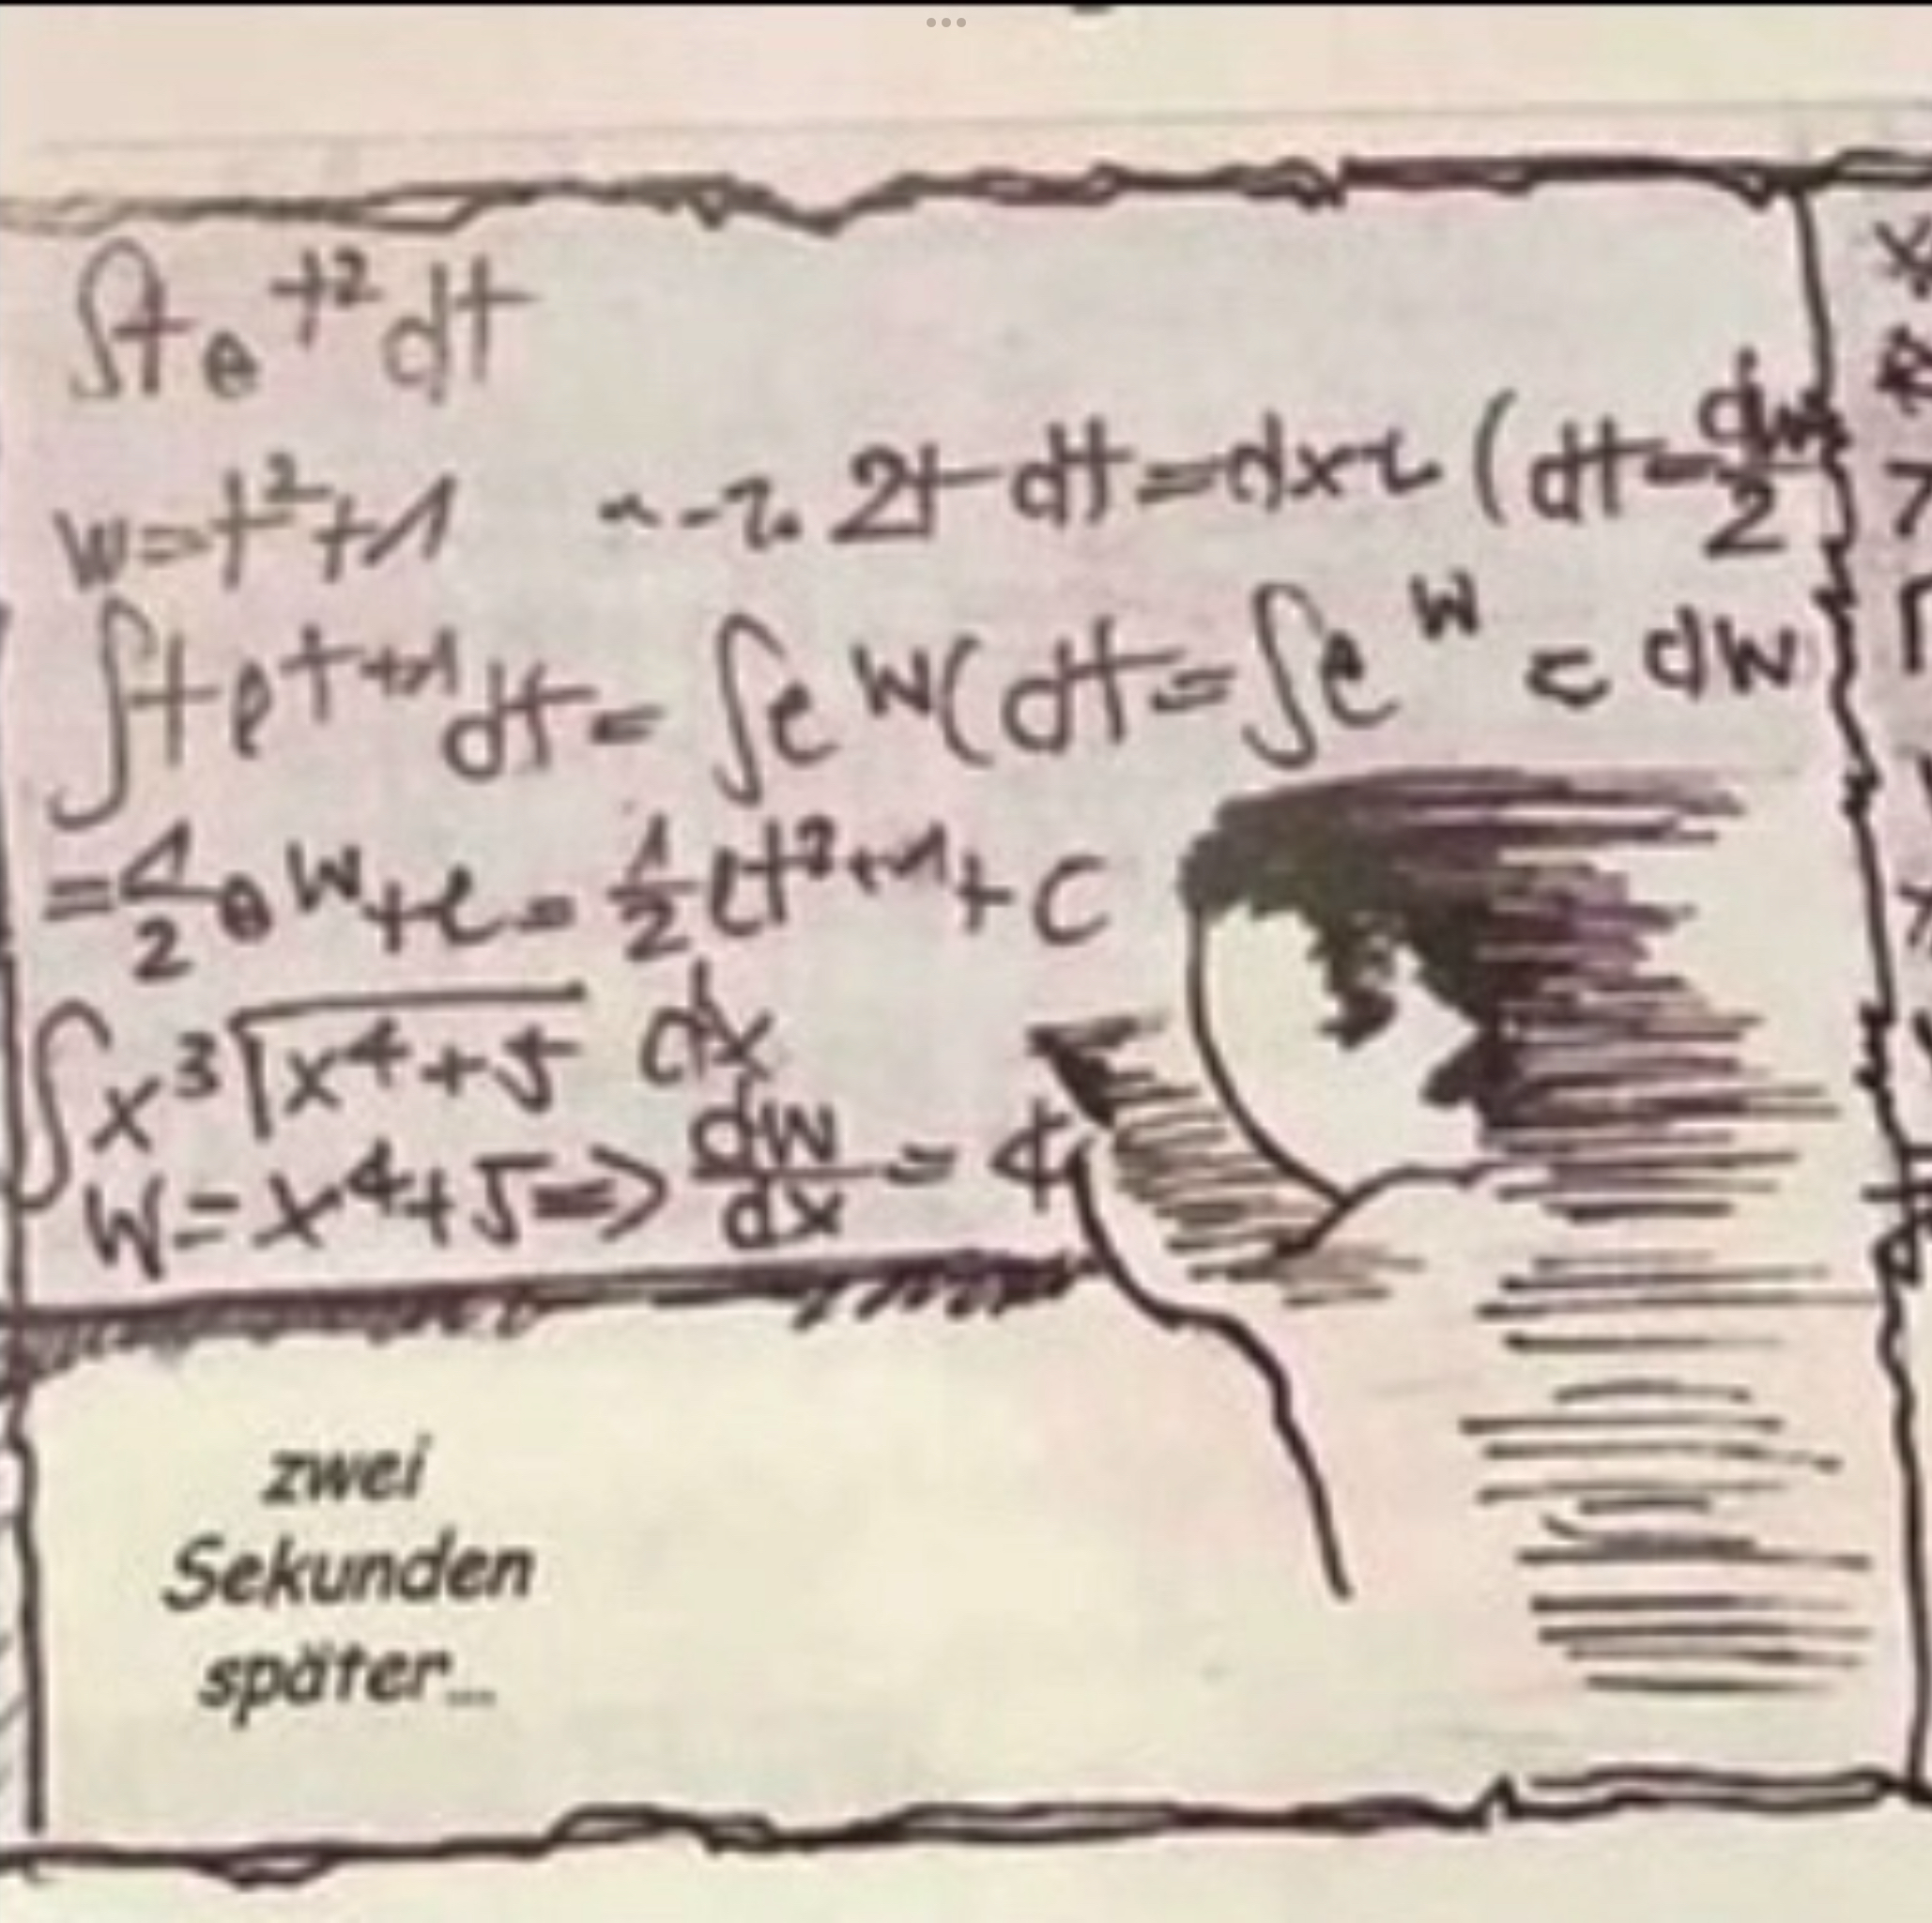
\includegraphics[width=1cm]{pictures/teacher_me_caricatur.png}}; % Adjust width and center image
\end{tikzpicture}}
}


\begin{document}
\maketitle
\thispagestyle{empty}
\cleardoublepage
\tableofcontents
\cleardoublepage

\pagestyle{headings}

\clearpage

\section{Bedingte Wahrscheinlichkeit}
\subsection{Tulpen aus Amsterdam}

\begin{wrapfigure}{r}{0.35\textwidth}
  \begin{center}
    \includegraphics[width=0.34\textwidth]{pictures/tulpen}
  \end{center}
%\caption{You Know my Name}
\end{wrapfigure}
Ein Hobbygärtner steckt $100$ Tulpenzwiebeln unter denselben Verhältnissen fachgerecht in den Boden. Nach einiger Zeit sind daraus $87$ herrliche Tulpen entstanden. Wenn man das Ereignis
\begin{itemize}
    \item[] A: aus der Zwiebel entsteht eine Tulpe
\end{itemize}
festlegt, so gilt für dieses Ereignis $P(A)=0.87$.
Der Hobbygärtner hatte nicht alle $100$ Zwiebeln bei demselben Händler gekauft. $60$ Zwiebeln stammten von einem Grossversand aus Holland, die restlichen $40$ Zwiebeln waren ein Sonderangebot aus einem Gartencenter. Bei genauerer Untersuchung stellte der Gärtner fest, dass von den $13$ Zwiebeln, die keine Tulpe hervorbrachten, nur deren $3$ aus Holland kamen und die restlichen Zwiebeln aus dem Gartencenter stammten. Der Grossversand aus Holland lieferte also mit $\nicefrac{57}{60}=95\%$ gute Zwiebeln, während das Sonderangebot aus dem Gartencenter nur $\nicefrac{30}{40}=75\%$ gute Zwiebeln ergab. Bezeichnet man das Ereignis
\begin{itemize}
    \item[] B: Zwiebel kommt aus Holland,
\end{itemize}
so gilt $P(B)=0.6$.
Die Wahrscheinlichkeit $P(A)=0.87$ sollte man präziser als die \emph{unbedingte} Wahrscheinlichkeit für das Entstehen einer schönen Tulpe bezeichnen. Mit dem Ereignis B zusammen lässt sich nämlich eine bedingte Wahrscheinlichkeit für A bilden; dies ist die Wahrscheinlichkeit, dass die Zwiebel eine Tulpe hervorbringt unter der Bedingung, dass sie aus Holland stammt. Man bezeichnet diese Wahrscheinlichkeit mit $P(A|B)$.
Aus den obigen Überlegungen ergab sich $P(A|B)=0.95$.

Diese bedingte Wahrscheinlichkeit darf nicht verwechselt werden mit der Wahrscheinlichkeit, aus einer Kiste mit allen $100$ noch nicht eingepflanzten Zwiebeln eine gute, aus Holland kommende Zwiebel zu ziehen, denn diese Wahrscheinlichkeit ist
$$P(A\cap B)=0.6\cdot0.95 = 0.57.$$
Man erkennt aber den Zusammenhang
$$P(A|B)\cdot P(B)=P(A\cap B).$$

\begin{table}[h]
\centering
\scalebox{0.8}{
\begin{tabular}{|l|c|c|c|}
\hline
\rowcolor{lightgray}\spaltenheight  & Holland & Gartencenter & \spaltensep \hline
\rowcolor{lightyellow}\spaltenheight Tulpe & 57 & 30 & 87\spaltensep \hline
\rowcolor{Gray}\spaltenheight keine Tulpe & 3 & 10 & 13\spaltensep \hhline{|====}
\rowcolor{lightyellow}\spaltenheight & 60 & 40 & 100\spaltensep \hline
\end{tabular}
}
\caption{Zuchterfolg bei Tulpen}\label{tab:tulpen}
\end{table}

Die Tabelle \ref{tab:tulpen} auf Seite \pageref{tab:tulpen} verdeutlicht noch einmal den Sachverhalt aus dem Beispiel.

\subsection{Einschränkung des Ereignisraumes}
\begin{cdef}[Bedingte Wahrscheinlichkeit]{}
Sei $\mathbb{B}$ ein Ereignis mit $P(\mathbb{B}) > 0$. Die Wahrscheinlichkeit des Eintretens des Ereignisses $\mathbb{A}$ unter der Bedingung, dass das Ereignis $\mathbb{B}$ bereits eingetreten ist, oder kurz, die \emph{bedingte Wahrscheinlichkeit} von $\mathbb{A}$ unter der Bedingung $\mathbb{B}$, $P(\mathbb{A}|\mathbb{B})$, wird definiert durch
$$P(\mathbb{A}|\mathbb{B}):=\frac{P(\mathbb{A}\cap\mathbb{B})}{P(\mathbb{B})}.$$
\end{cdef}

\begin{bem}
$P(A|B)$ ist die relative Wahrscheinlichkeit von A bezüglich des \emph{reduzierten} Stichprobenraumes B.
\end{bem}

\begin{ueb}[Tulpen aus Amsterdam]
A und B seien die Ereignisse aus dem Einführungsbeispiel.
\begin{enumerate}[a)]
\item Zeige: $P(A)=P(A\cap B) +P(A\cap\overline{B})$.
\item Berechne $P(B|A)$. (Man sieht eine herrliche Tulpe. Gesucht ist die Wahrscheinlichkeit, dass die zugehörige Zwiebel in Holland gekauft wurde.)
%\item Interpretiere und berechne $P(\overline{A}|B)$, $P(A|\overline{B})$, $P(\overline{A}|\overline{B})$, $P(B|A)$, $P(B|\overline{A})$ und $P(\overline{B}|\overline{A})$.
%\item Bestätige $P(A)\cdot P(B|A) = P(B)\cdot P(A|B)$.
%\item Ist die Aussage $P(A|B) = 1 - P(\overline{A}|B)$ richtig?
\end{enumerate}
\end{ueb}

\begin{ueb}[Lügendetektortest]
Ein Lügendetektor-Test entscheide in 90\% aller Fälle richtig, sowohl bei Schuldigen, als auch bei Unschuldigen. Um Diebstähle zu reduzieren, entlässt eine grosse Firma alle Angestellten, die beim Test durchfallen. Vor der Entlassungsaktion seien 5\% aller Angestellten Diebe.
\begin{enumerate}[a)]
\item Wie viele unter den Entlassenen wären tatsächlich Diebe?
\item Wie viele Diebe würden nicht erfasst?
\end{enumerate}
\end{ueb}

%\begin{ueb}[Kaffeetrinker im Orchester]
%In einem Orchester spielen 40 Personen. Drei Fünftel aller Personen trinken gerne Kaffee, darunter 15 der 25 männlichen Orchestermitglieder.
%\begin{enumerate}[a)]
%\item Bestimme die Wahrscheinlichkeit dafür, dass ein zufällig ausgewähltes Orchestermitglied,
%\begin{enumeratei}
%\item weiblich ist.
%\item weiblich ist oder nicht gerne Kaffee trinkt.
%\end{enumeratei}
%\item Bestimme die Wahrscheinlichkeit dafür, dass ein zufällig ausgewähltes Orchestermitglied männlich ist,
%wenn bekannt ist, dass er nicht gerne Kaffee trinkt.
%\end{enumerate}
%\end{ueb}

\begin{ueb}[Sensitivität und Spezifität]
Schreibe auf, was die Begriffe \emph{Sensitivität} und \emph{Spezifität} bedeuten. Kontrolliere deine Aussagen mithilfe der Angaben aus dem Skript auf Seite \pageref{ueb:hiv} (\"Ubung HIV Test).
\end{ueb}

\begin{ueb}[Covid-19 Selbsttest]
Betrachte die Angaben zur Sensitivität und Spezifität auf dem folgenden Ausschnitt des Beipackzettels eines gängigen Tests (Abbildung \ref{fig:covidchart} auf Seite \pageref{fig:covidchart})

\begin{figure}
    \centering
    \includegraphics[width=0.618\textwidth]{pictures/Covidchart.jpeg}
    \caption{Beipackzettel Covid-19 Selbsttest}
    \label{fig:covidchart}
\end{figure}

\begin{enumerate}[a)]
    \item Bestimme die Spezifität und die niedrigste der angegebenen Sensitivitäten.
\end{enumerate}
Nimm an, dass aktuell $5\%$ der Bevölkerung an Covid-19 erkrankt ist.
\begin{enumerate}[a)]
\setcounter{enumi}{1}
    \item Berechne die Wahrscheinlichkeit, dass eine zufällig  ausgewählte Person  tatsächlich krank ist, wenn der Test positiv anzeigt (\emph{positiv prädiktiver Wert}).
    \item Berechne die Wahrscheinlichkeit, dass eine zufällig ausgewählte Person tatsächlich gesund ist, wenn der Test negativ anzeigt (\emph{negativ prädiktiver Wert}).
\end{enumerate}
Seien wir jetzt in einer Pandemie und gesch\"atzte $20\%$ der Bev\"olkerung sei an Covid-19 erkrankt. Wir testen eine ganze Schule (ca. 1000 Personen).
\begin{enumerate}[a)]
\setcounter{enumi}{3}
    \item Erstelle dazu ebenfalls eine geeignete Tabelle mit den Werten für die richtig positiven, die falsch positiven, die richtig negativen und die falsch negativen Tests.
Wie viele kranke Personen werden nicht erkannt?
\end{enumerate}
\end{ueb}

\begin{ueb}[geringe Spezifität]
Die Corona Selbsttests haben eine sehr hohe Spezifität und eine hohe Sensitivität. Was bedeutet es für Patienten, wenn ein medizinischer Test eine hohe Sensitivität, aber eine nicht so hohe Spezifität hat?
\end{ueb}

\begin{ueb}[Selbsttest 2020]
Im Anhang C im Skript findest du Angaben zu zwei verschiedenen Covid-19 Selbsttests aus dem Jahr 2020.
\begin{enumerate}[a)]
    \item Rechne die Werte für die positive und negative Prädikation nach.
\end{enumerate}
Die Sensitivität ist bei diesen Tests deutlich tiefer als beim neuen Test, auch die Spezifität ist beim zweiten Test niedriger.
\begin{enumerate}[a)]
\setcounter{enumi}{1}
\item Wären die Testergebnisse für die ganze Schule genauso gut oder gar schlechter verglichen mit dem neuen Test? Erstelle dazu dieselben Tabellen wie in Aufgabe 2e).
\end{enumerate}
\end{ueb}

\begin{ueb}[HIV Test]
\label{ueb:hiv}
Zur
\marginnote{
\qrcode{
https://www.youtube.com/watch?v=r8b7m2YHgL0}
}
Beurteilung eines HIV-Tests seien folgende Werte gegeben. Die Wahrscheinlichkeit, dass jemand HIV positiv ist, beträgt $1\div10\,000$; also

$$P(H):=0.01\%.$$

Ferner kenne man die \emph{Sensitivität} (Wahrscheinlichkeit, dass der Test positiv anzeigt, falls die Person tatsächlich positiv ist.):
$$P(p|H)=99.9\%$$
und die \emph{Spezifität} (Wahrscheinlichkeit, dass der Test negativ anzeigt, falls die Person tatsächlich negativ ist.):
$$P(\bar{p}|\bar{H})=99.7\%.$$

\begin{enumerate}[a)]
\item Berechne die Wahrscheinlichkeit, dass eine zufällig ausgewählte Person tatsächlich HIV positiv ist, wenn sie ein positives Testresultat erhalten hat.\footnote{definiert als: \emph{positiv prädiktiver Wert}} Schätze diese Wahrscheinlichkeit zuerst.
\item Berechne die Wahrscheinlichkeit, dass eine zufällig ausgewählte Person tatsächlich negativ ist, unter der Voraussetzung, dass sie ein negatives Testergebnis erhalten hat.\footnote{definiert als: \emph{negativ prädikitiver Wert}}
\end{enumerate}

\end{ueb}

%\begin{ueb}[Alleskönner, Besserwisser, Chancenlos]
%Eine Firma beschäftigt drei Mitarbeiter, die telefonische Anfragen von Kunden beantworten sollen. Herr Alleskönner kann 90\% aller Frage zur Zufriedenheit der Kunden beantworten, Frau Besserwisser 80\% und Herr Chancenlos noch gerade 70\%. Berechnen Sie unter der Annahme, dass alle drei Mitarbeiter gleich viele Telefonate beantworten, die Wahrscheinlichkeiten, dass

%\begin{enumerate}[a)]
%\item ein Kunde an Herrn Alleskönner gerät und eine zufrieden stellende Antwort bekommt.
%\item ein Kunde an Herrn Chancenlos gerät und eine nicht zufrieden stellende Antwort
%bekommt.
%\item ein Kunde mit der Antwort, die er erhält, nicht zufrieden ist.
%\item ein unzufriedener Kunde an Frau Besserwisser geraten ist.
%\item eine Antwort, die zur Zufriedenheit des Kunden ausfiel, von Herrn Chancenlos
%gegeben wurde.
%\item eine Antwort, die den Kunden nicht zufrieden stellt, von Herrn Alleskönner gegeben
%wurde.
%\end{enumerate}
%\end{ueb}

\begin{ueb}[Wer steckt unter dem Tirolerhut]
In einem bayrischen Touristenort sind zur Hochsaison drei Mal so viele Touristen wie Einheimische. Touristen tragen zu 70\% einen Tirolerhut, Einheimische nur zu 25\%.
\begin{enumerate}[a)]
\item Du fragst einen Menschen mit Tirolerhut nach dem Weg. Wie groß ist die Wahrscheinlichkeit, dass der
Mensch ein Einheimischer ist?
\item Du fragst einen Menschen ohne Tirolerhut nach dem Weg. Wie groß ist die Wahrscheinlichkeit, dass
der Mensch ein Einheimischer ist?
\end{enumerate}
Was ist also günstiger, wenn du möglichst schnell eine verlässliche Wegauskunft haben möchtest?
\end{ueb}

%\begin{ueb}
%Eine Krankheit kommt in der Bevölkerung mit einer Wahrscheinlichkeit von $2\%$ vor. Der Test für die Krankheit ist zurzeit noch sehr unsicher, er zeigt nämlich sowohl für die Kranken wie auch die Gesunden ihren Zustand mit einer Sicherheit von 75\% an.

%\begin{enumerate}[a)]
%%\item Der Test zeigt für eine Person das Vorhandensein der Krankheit an. Wie gross ist die
%Wahrscheinlichkeit, tatsächlich krank zu sein?
%\item Die Firma möchte nun durch weitere Investitionen den Test genauer machen. Du
%sollst entscheiden, ob die Investitionen eher in die genauere Indikation bei den
%Kranken oder bei den Gesunden fliessen soll. Rechne dazu die Situation unter (a) durch, wenn die Genauigkeit
%\begin{enumeratei}
%\item für die Kranken (die Sensitivität) von 75\% auf 90\% gesteigert wurde.
%\item für die Gesunden (die Spezifität) von 75\% auf 90\% gesteigert wurde.
%\end{enumeratei}
%Wohin sollte also die Investition fliessen?
%\end{enumerate}
%\end{ueb}

Im Anhang \ref{appendix:aerztecovid} gegen Ende des Skripts (Seite \pageref{appendix:aerztecovid}) kann man Zahlen aus einem Ärzte-Communiqué zu einem neuen Covid19 Schnelltest, der damals im Nov 2020 eingeführt wurde, nachrechnen.

\begin{figure}
    \centering
    \includegraphics[width=0.35\textwidth]{pictures/bedingtewkeit.png}
    \caption{You're probabely near the ocean.}
\end{figure}

\subsection{Unabhängigkeit}

Ein Ereignis A heisst \emph{unabhängig} von einem Ereignis B, wenn das Eintreten von B die Wahrscheinlichkeit für das Eintreten von A nicht beeinflusst, d.h. wenn die Wahrscheinlichkeit von A gleich der bedingten Wahrscheinlichkeit von A unter der Bedingung B ist. Diese Gleichung führt zu

\begin{cdef}[Unabhängigkeit]{}
Zwei Ereignisse A und B heissen \emph{unabhängig}, wenn
$$P(A\cap B) = P(A)\cdot P(B),$$
andernfalls heissen sie \emph{abhängig}.
\end{cdef}

%\begin{ueb}[Chemie und Physik]
%Bei der ersten Vorprüfung der Mediziner sind $25\%$ der Kandidaten in Physik, $15\%$ in Chemie und $10\%$ in Physik und Chemie durchgefallen. Wie gross ist die Wahrscheinlichkeit, dass ein zufällig ausgewählter Kandidat
%\begin{enumerate}[a)]
%\item in Physik durchfiel, wenn man weiss, dass er in Chemie nicht bestanden hat?
%\item in Chemie durchfiel, wenn man weiss, dass er in Physik nicht bestanden hat?
%\item in Physik oder Chemie durchfiel?
%\end{enumerate}
%\end{ueb}

\begin{ueb}[Blutgruppen und Geschlecht]
Zur Untersuchung, ob die vier Hauptblutgruppen 0, A, B, AB vom Geschlecht abhängen, wurden die für Mitteleuropa gültigen Daten in der Tabelle \ref{blutgrp} auf Seite \pageref{blutgrp} erhoben. Kann man daraus schliessen, dass die Verteilung der Blutgruppen vom Geschlecht unabhängig ist?

\begin{table}[h]
\begin{center}
\begin{tabular}{|l|c|c|c|c||c|}
\hline
\rowcolor{Gray}\spaltenheight & 0 & A & B & AB & \spaltensep \hhline{|-|-|-|-|--|}
\rowcolor{lightyellow}\spaltenheight  weiblich & 817 & 723 & 176 & 92 & 1808\spaltensep \hhline{|-|-|-|-|--|}
\rowcolor{Gray}\spaltenheight  männlich & 862 & 765 & 191 & 106 & 1924\spaltensep \hhline{|=|=|=|=|=#=|}
\rowcolor{lightyellow}\spaltenheight   & 1679 & 1488 & 367 & 198 & 3732\spaltensep \hline
\end{tabular}
\end{center}
\caption{Blutgruppen und Geschlechter}\label{blutgrp}
\end{table}
\end{ueb}

\begin{ueb}[rothaarig und Geschlecht]
Gibt
\marginnote{
\qrcode{
https://www.youtube.com/watch?v=VIZhN7IbuiA}
}
es eine Abhängigkeit zwischen Haarfarbe und Geschlecht? Diskutiere dies aufgrund der Daten aus Tabelle \ref{Haarfarbe} auf Seite \pageref{Haarfarbe}, die aus einem nordeuropäischen Land stammen.

\begin{table}[h]
\begin{center}
\begin{tabular}{|l|c|c|c|c|}
\hline
\rowcolor{Gray}\spaltenheight & hellblond & dunkelblond & rot & schwarz\spaltensep \hline
\rowcolor{lightyellow}\spaltenheight  weiblich & 195 & 121 & 38 & 67\spaltensep \hline
\rowcolor{Gray}\spaltenheight  männlich & 110 & 199 & 236 & 59\spaltensep \hline
\end{tabular}
\end{center}
\caption{Testresultat Haarfarbe}\label{Haarfarbe}
\end{table}
\end{ueb}

\begin{ueb}[Ziegenproblem]
In
\marginnote{
\qrcode{
https://youtu.be/_i1VTQKpGHQ}
}
einer Gameshow befinden sich hinter drei Türen A, B und C ein Auto und zwei Ziegen. Die Kandidatin wählt Tür A, der Showmaster öffnet Tür C, hinter der sich eine Ziege befindet. Dann bietet er der Kandidatin an, eventuell die Tür B zu wählen. Soll sie?
\end{ueb}

\clearpage

\section{Zufallsgrössen \& Lageparameter}

\subsection{Zufallsvariable}
\begin{wrapfigure}{r}{0.382\textwidth}
  \begin{center}
    \includegraphics[width=0.3\textwidth]{pictures/bandit}
  \end{center}
%\caption{You Know my Name}
\end{wrapfigure}
Glücksspiele nennt man gerecht (fair), günstig oder ungünstig, je nachdem, ob der Gewinn, den man bei mehreren Spielen erwarten kann, $=0, >0$, oder $<0$ ist. Zur Analyse eines Glücksspiels muss man von allen möglichen Ausgängen $\omega_i$ die entsprechenden Wahrscheinlichkeiten $P(\omega_i)$ und die zugehörigen positiven oder negativen Gewinne kennen.

\begin{bsp}
Als charakteristisches Beispiel wählen wir ein intuitiv gerechtes Spiel: Peter und Paul werfen je einen Fünfliber; bei gleichen Wurfbildern gewinnt Peter, andernfalls Paul beide Münzen.
Die Tabelle \ref{tab:5liber} auf Seite \pageref{tab:5liber} enthält alle zur Analyse wichtige Daten.

\begin{table}
\begin{center}
\begin{tabular}{|c|c|c|c|c|}
\hline
\rowcolor{Gray}\spaltenheight $\omega_i\in\Omega$ & 00 & 01 & 10 & 11\spaltensep \hline
\rowcolor{lightyellow}\spaltenheight $P(\omega_i)$ & $\frac{1}{4}$ & $\frac{1}{4}$ & $\frac{1}{4}$ & $\frac{1}{4}$\spaltensep \hline
\rowcolor{Gray}\spaltenheight Peters Gewinn & $5$ & $-5$ & $-5$ & $5$\spaltensep \hline
\end{tabular}
\end{center}
\caption{Gewinn aus Peters Sicht beim Fünfliber-Spiel}\label{tab:5liber}
\end{table}
\end{bsp}
Aus dieser Tabelle lässt sich sofort eine Funktion $X:\omega_i\mapsto X(\omega_i)$
erkennen. Diese Funktion ordnet jedem Ausgang $\omega_i$ den zugehörigen Gewinn oder Verlust zu.

\begin{cdef}[Zufallsvariable]{}
Eine Funktion, deren Definitionsmenge der Stichprobenraum $\Omega$ ist und deren Wertemenge die reellen Zahlen sind
$$X:\Omega \to \mathbb{R}$$
nennt man eine \emph{Zufallsvariable}.
\end{cdef}

\begin{bem}
Der Name ist historisch bedingt. Eine Zufallsvariable ist eigentlich weder zufällig noch variabel, sondern eine reelle Zahlenfunktion. Derartige Funktionen werden üb\-li\-cher\-wei\-se mit grossen Buchstaben X, Y, Z bezeichnet.
Beachten Sie ebenfalls die Unterschiede zur Wahrscheinlichkeitsfunktion.
\end{bem}

Man bezeichnet die Funktionswerte der Zufallsvariablen $X$ mit $x_1, x_2, x_3, \dots$ und konzentriert sich auf die Wahrscheinlichkeiten, mit denen die einzelnen Funktionswerte angenommen werden. Zu diesem Zweck erstellt man eine neue Tabelle, die die \emph{Wahrscheinlichkeitsverteilung} der Zufallsvariablen X angibt.

\begin{table}
\begin{center}
\begin{tabular}{|c|c|c|}
\hline
\rowcolor{Gray}\spaltenheight $\q x_i\q$ & $\q5\q$ & $\q-5\q$\spaltensep \hline
\rowcolor{lightyellow}\spaltenheight $P(X=x_i)$ & $0.5$ & $0.5$\spaltensep \hline
\end{tabular}
\end{center}
\caption{Gewichtung der Zufallsvariablen beim Fünfliber-Spiel}
\end{table}

Mit dieser Wahrscheinlichkeitsverteilung der Zufallsvariablen X lässt sich der Durchschnittswert je Spielwiederholung berechnen. Dazu muss man jeden Gewinn mit der entsprechenden Wahrscheinlichkeit gewichten: Durchschnittsgewinn entspricht $5\cdot0.5 + (-5)\cdot0.5 = 0$.
Unser Gefühl, dass es sich um ein gerechtes Spiel handelt, also bei vielen Wiederholungen weder Gewinn noch Verlust zu erwarten ist, wird somit rechnerisch bestätigt.

\subsection{Erwartungswert}

\begin{cdef}[Erwartungswert]{}
Allgemein bezeichnet man das mit den entsprechenden Wahrscheinlichkeiten gewichtete Mittel der Funktionswerte der Zufallsvariablen X als den \emph{Erwartungswert}:
$$E(X)= x_1\cdot P(X=x_1) + x_2\cdot P(X=x_2)+\dots.$$
\end{cdef}

\begin{bsp}
Zwei Würfel werden sehr oft geworfen. Welche Augensumme darf man durchschnittlich erwarten? Die Zufallsvariable X ordnet jedem 
$$\omega_i\in\Omega=\set{11,12,\dots,16,\dots,66}$$
die Augensumme der beiden Würfel zu. Die möglichen Funktionswerte der Zufallsvariablen sind $x_1=2$, $x_2=3$, $x_3=4$, \dots, $x_{11}=12$.

\begin{ueb}[Relative Häufigkeiten]
Ergänze in Tabelle \ref{tab:wuerfeln} auf Seite \pageref{tab:wuerfeln} die Wahrscheinlichkeitsverteilung.

\begin{table}
\begin{center}
\begin{tabular}{|c|c|c|c|c|c|c|}
\hline
\rowcolor{Gray}\spaltenheight $\;\; x_i\;\;$ & $\;\;2\;\;$ & $\;\;3\;\;$ & $\;\;4\;\;$ & $\;\;5\;\;$ & $\;\;6\;\;$ & $\;\;7\;\;$\spaltensep \hline
\rowcolor{lightyellow}\rule{0mm}{3ex} $P(X=x_i)$ &  & & & & & \\[3ex] \hline
\rowcolor{Gray}\spaltenheight $\;\; x_i\;\;$ & $\;\;8\;\;$ & $\;\;9\;\;$ & $\;10\;$ & $\;11\;$ & $\;12\;$ & \phantom{$\;12\;$}\spaltensep \hline
\rowcolor{lightyellow}\rule{0mm}{3ex} $P(X=x_i)$ &  & & & & & \\[3ex] \hline
\end{tabular}
\end{center}
\caption{Wahrscheinlichkeitsverteilung beim Werfen von zwei Würfeln}\label{tab:wuerfeln}
\end{table}
\end{ueb}

Beachten Sie, dass die Summe aller Wahrscheinlichkeiten 100\% beträgt. Für den Erwartungswert ergibt sich dann
$$E(X) = \frac{1}{36}\cdot(2\cdot1 + 3\cdot2 + 4\cdot3 + \ldots + 11\cdot2 + 12\cdot1) = 7.$$
Die	Wahrscheinlichkeitsverteilung wird durch ein Stabdiagramm dargestellt. Für den Wurf mit zwei Würfeln ergibt sich das Bild \ref{abb:hkeitwuerfel} auf Seite \pageref{abb:hkeitwuerfel}.

\begin{figure}[h]
\centering
\definecolor{zzttqq}{rgb}{0.6,0.2,0}
\begin{tikzpicture}[line cap=round,line join=round,>=triangle 45,x=0.7cm,y=0.7cm]
\draw[->,color=black] (-1.16,0) -- (13.9,0);
\foreach \x in {2,3,4,5,6,7,8,9,10,11,12}
\draw[shift={(\x,0)},color=black] (0pt,2pt) -- (0pt,-2pt) node[below] {\footnotesize $\x$};
\draw[color=black] (13.5,0.08) node [anchor=south west] {$x_i$};
\draw[->,color=black] (0,-1.18) -- (0,7.34);
\foreach \y in {1,2,3,4,5,6}
\draw[shift={(0,\y)},color=black] (2pt,0pt) -- (-2pt,0pt) ;
\draw[color=black] (0.1,6.94) node [anchor=west] {$P(X=x_i)$};
\draw[color=black] (-1.3,6) node [anchor=west] {$\frac{6}{36}$};
\draw[color=black] (-1.3,1) node [anchor=west] {$\frac{1}{36}$};
\clip(-0.6,-0.6) rectangle (13.9,7.34);
\draw[line width=2pt,color=zzttqq,fill=zzttqq,fill opacity=0.15] (2,0) rectangle (2,1);
\draw[line width=2pt,color=zzttqq,fill=zzttqq,fill opacity=0.15] (3,0) rectangle (3,2);
\draw[line width=2pt,color=zzttqq,fill=zzttqq,fill opacity=0.15] (4,0) rectangle (4,3);
\draw[line width=2pt,color=zzttqq,fill=zzttqq,fill opacity=0.15] (5,0) rectangle (5,4);
\draw[line width=2pt,color=zzttqq,fill=zzttqq,fill opacity=0.15] (6,0) rectangle (6,5);
\draw[line width=2pt,color=zzttqq,fill=zzttqq,fill opacity=0.15] (7,0) rectangle (7,6);
\draw[line width=2pt,color=zzttqq,fill=zzttqq,fill opacity=0.15] (8,0) rectangle (8,5);
\draw[line width=2pt,color=zzttqq,fill=zzttqq,fill opacity=0.15] (9,0) rectangle (9,4);
\draw[line width=2pt,color=zzttqq,fill=zzttqq,fill opacity=0.15] (10,0) rectangle (10,3);
\draw[line width=2pt,color=zzttqq,fill=zzttqq,fill opacity=0.15] (11,0) rectangle (11,2);
\draw[line width=2pt,color=zzttqq,fill=zzttqq,fill opacity=0.15] (12,0) rectangle (12,1);
\end{tikzpicture}
\caption{Häufigkeitsverteilung beim Würfeln mit zwei Würfel}\label{abb:hkeitwuerfel}
\end{figure}

\end{bsp}

\begin{ueb}[Der Zufall regiert die Welt]
Aus einer Urne mit fünf Kärtchen
$$\set{\texttt{DER, ZUFALL, REGIERT, DIE, WELT}}$$
wird ei\-nes der fünf Wörter zufällig gezogen. Berechne den Er\-war\-tungs\-wert der Zu\-fall\-svaria\-blen
\begin{enumerate}[a)]
\item W, deren Funktionswerte die Länge des gewählten Wortes angeben,
\item V, deren Funktionswerte die Anzahl der Vokale im gewählten Wort angeben,
\item X, deren Funktionswerte die Anzahl \texttt{e} im gewählten Wort angeben.
\end{enumerate}
\end{ueb}

\begin{ueb}[9 dritteln oder verdreifachen]
Du hast jetzt 9 Franken. Eine Münze wird geworfen. Erscheint \glqq Kopf\grqq, wird dein Vermögen verdreifacht, erscheint \glqq Zahl\grqq, wird dein Vermögen gedrittelt. Welches Vermögen darfst du nach zweimaligem Werfen erwarten?
\end{ueb}

\begin{ueb}[Chuck a Luck]
In amerikanischen Casinos findet das Würfelspiel \emph{Chuck a Luck} grossen Anklang. Der Spieler darf auf eine der Zahlen $1$, $2$, $3$, $4$, $5$, $6$ setzen. Dann werden drei Würfel geworfen. Erscheint seine Zahl ein-, zwei- oder dreimal, so erhält er das ein-, zwei- oder dreifache seines Einsatzes und dazu seinen Einsatz zurück. Andernfalls verliert er natürlich seinen Einsatz. Berechne den zu erwartenden Gewinn bei einem Einsatz von 10\$.
\end{ueb}

\begin{ueb}[Einarmiger Bandit]
Ein Glücks\-spiel\-apparat hat zwei Räder, die der Spieler durch Hebeldruck in Bewegung setzen kann. Auf jedem Rad sind vier Glocken, fünf Kirschen und ein Apfel in regelmässigen Abständen abgebildet. Der Apparat zahlt für zwei Äpfel Fr. 10.-, für zwei Glocken Fr. 2.- und für zwei Kirschen Fr. 1.- und man kriegt den Einsatz zurück. Der
Einsatz beträgt Fr. 1.-. Wer gewinnt hier?
\end{ueb}

\begin{ueb}[five all, quiet please!]
Zwei
\marginnote{
\qrcode{
https://youtu.be/UQ8p6NywTvA}
}
gleich starke Tennisspieler müssen den Sieg in einem Tie-Break entscheiden. Es steht bereits 5:5. Wie viele Punkte müssen voraussichtlich noch bis zur Entscheidung gespielt werden?
\end{ueb}

\subsection{Standardabweichung}

Als Kennzahl für einen zu erwartenden Wert haben wir bereits den Erwartungswert. Im Folgenden wollen wir eine Masszahl für die \emph{Streuung} um diesen Erwartungswert kreieren.

\begin{bsp}
Zwei Maschinen A und B schneiden bei einem Probelauf Stahlstifte auf eine vorgegebene Länge von $\unit[10.0]{mm}$ zu. Untersuchungen über auftretende Abweichungen ergaben folgende Wahrscheinlichkeitsverteilungen für die anfallenden Längen:
\begin{center}
\begin{minipage}{7.5cm}
\centering\emph{Maschine A}\\[2ex]
\begin{tabular}{|c|c|c|c|c|c|}
\hline
\rowcolor{Gray}\spaltenheight $x_i$ & 9.8 & 9.9 & 10.0 & 10.1 & 10.2\spaltensep \hline
\rowcolor{lightyellow}\spaltenheight $P(X=x_i)$ & 0.1 & 0.1 & 0.6 & 0.1 & 0.1\spaltensep \hline
\end{tabular}
\end{minipage}

\vspace*{2ex}
\begin{minipage}{7.5cm}
\centering\emph{Maschine B}\\[2ex]
\begin{tabular}{|c|c|c|c|c|c|}
\hline
\rowcolor{Gray}\spaltenheight $y_i$ & 9.8 & 9.9 & 10.0 & 10.1 & 10.2\spaltensep \hline
\rowcolor{lightyellow}\spaltenheight $P(Y=y_i)$ & 0.1 & 0.2 & 0.4 & 0.2 & 0.1\spaltensep \hline
\end{tabular}
\end{minipage}
\end{center}

\begin{ueb}[Werte, Erwartungswerte und Abweichungen]
Stelle beide Verteilungen mit verschiedenen Farben im Koordinatensystem \ref{koordsys} graphisch dar und berechne die Erwartungswerte $E(X)$ und $E(Y)$.
\end{ueb}

\begin{figure}[h]
\centering
\definecolor{cqcqcq}{rgb}{0.75,0.75,0.75}
\begin{tikzpicture}[line cap=round,line join=round,>=triangle 45,x=0.8cm,y=0.7cm]
\draw [color=cqcqcq,dash pattern=on 3pt off 3pt, xstep=0.8cm,ystep=0.7cm] (0,0) grid (11.5,7.5);
\draw[->,color=black] (-0.84,0) -- (12.06,0);
\foreach \x in {1,2,3,4,5,6,7,8,9,10,11}
\draw[shift={(\x,0)},color=black] (0pt,2pt) -- (0pt,-2pt);
\draw[color=black] (11.72,0.08) node [anchor=south west] {$x_i,y_i$};
\draw[->,color=black] (0,-0.64) -- (0,7.72);
\foreach \y in {1,2,3,4,5,6,7}
\draw[shift={(0,\y)},color=black] (2pt,0pt) -- (-2pt,0pt) node[left] {\footnotesize $0.\y$};
\draw[color=black] (0.1,7.32) node [anchor=west] {$P$};
\draw[color=black] (6,-0.1) node [anchor=north] {$10.0$};
\clip(-0.84,-0.64) rectangle (12.06,7.72);
\end{tikzpicture}
\caption{Relative Genauigkeit der Maschinen A und B}\label{koordsys}
\end{figure}
\end{bsp}
Obwohl die graphischen Darstellungen ganz verschieden aussehen, stimmen die Erwartungswerte mit dem Sollwert überein. Offensichtlich wird man aber die Maschine A bevorzugen.
Der Erwartungswert gibt nur an, wo das \emph{Zentrum} der Verteilung liegt, nicht aber, wie stark die Verteilung \emph{um ihr Zentrum konzentriert} ist. Deshalb benötigt man eine Masszahl für die Abweichung der Funktionswerte der Zufallsvariablen von ihrem Erwartungswert.

In der deskriptiven Statistik haben wir die Standardabweichung $s$ kennengelernt. Um für die Zufallsvariable $X$ ein entsprechendes Streuungsmass zu erhalten, muss man sinngemäss den Mittelwert $\bar{x}$ durch den Erwartungswert $E(X)$, die einzelnen Messwerte $x_i$ durch die Funktionswerte der Zufallsvariablen $X$ und die relativen Häufigkeiten ($\frac{1}{n}$ bzw. $\frac{n_i}{n}$) durch die Wahrscheinlichkeiten $P(X=x_i)$ ersetzen.

\begin{cdef}[Standardabweichung]{}
Der Ausdruck
$$\sigma=\sqrt{(E(X)-x_1)^2\cdot P(X=x_1)+\dots+(E(X)-x_n)^2\cdot P(X=x_n)}$$
ist die \emph{Standardabweichung} der Zufallsvariablen $X$.
\end{cdef}
\marginnote{
\qrcode{
https://youtu.be/esGICLO0G8w}
}

\begin{ueb}[Standardabweichung berechnen]
Berechne für beide Maschinen aus dem obigen Beispiel die Standardabweichung der Zufallsvariablen $X$ und $Y$ und bestätige somit, dass die Maschine A zu bevorzugen ist.
\end{ueb}

\begin{ueb}[Blutdruck Medikament]
Der Blutdruck in der Oberarmschlagader eines gesunden Menschen beträgt etwa $\unit[120]{mm}$ Quecksilbersäule. Eine Arzneimittelfirma lässt zwei Medikamente A und B zur Regulierung des Blutdrucks klinisch testen. Die Ergebnisse sind in der Tabelle festgehalten:
\begin{table}[h]
\centering
\scalebox{1}{
\begin{tabular}{|c|c|c|c|c|c|c|c|c|}
\hline
\rowcolor{Gray}\spaltenheight & $x_i,y_i$ & 105 & 110 & 115 & 120 & 125 & 130 & 135 \spaltensep \hline
\rowcolor{lightyellow}\spaltenheight A: & $P(X=x_i)$ & 0.04 & 0.09 & 0.16 & 0.40 & 0.20 & 0.07 & 0.04\spaltensep \hline
\rowcolor{Gray}\spaltenheight B: & $P(Y=y_i)$ & 0.02 & 0.08 & 0.15 & 0.46 & 0.23 & 0.04 & 0.02\spaltensep \hline
\end{tabular}
}
\caption{Medikamententest}
\end{table}
Berechne für jedes Medikament den Erwartungswert und die Standardabweichung. Welches Medikament ist demnach vorteilhafter?
\end{ueb}

\clearpage

\section{Binomialverteilung}

Bei vielen Zufallsversuchen gibt es nur zwei mögliche Ausgänge: Mit einer Münze wirft man \glqq Kopf\grqq\ oder \glqq Zahl\grqq, die gewürfelte Augenzahl ist eine $6$ oder keine $6$, die gezogene Karte ist ein Ass oder kein Ass, die Geburt eines Kindes ergibt eine Tochter oder einen Sohn, die Herzoperation gelingt oder gelingt nicht, \dots

\begin{cdef}[Binomialverteilung]{}
Ein Zufallsversuch mit genau zwei Ausgängen, also mit dem Stichprobenraum $\Omega=\{\text{Erfolg, Misserfolg}\}$ oder kurz $\set{1,0}$, heisst \emph{Bernoulli-Versuch}.
Man nennt in diesem Zusammenhang eine Zufallsvariable \emph{binomialverteilt} (lat. binominis, zweinamig).
\end{cdef}

\textsc{Jakob Bernoulli} (1759 -- 1809) war der erste Mathematiker, der die Wahrscheinlichkeitsprobleme, die aus dieser Art von Versuchen entstehen, systematisch untersuchte.
Üblicherweise wird die Wahrscheinlichkeit für einen Erfolg mit $p$ und die für einen Misserfolg mit $q$ bezeichnet: $P(1) = p$, $P(0) = q$, und damit $p + q = 1$.

Ein Bernoulli-Versuch werde $n$-mal wiederholt. Man spricht von einem $n$-stufigen Ber\-noul\-li-Ver\-such, wenn
\begin{itemize}
\item bei jeder Wiederholung des Bernoulli-Versuchs nur zwei Ausgänge möglich sind,
\item $P(1) = p$ bei jeder Wiederholung \emph{konstant} bleibt,
\item die einzelnen Wiederholungen des Bernoulli-Versuchs von\-einan\-der unab\-hän\-gig sind.
\end{itemize}
Bei einem $n$-stufigen Bernoulli-Versuch interessiert man sich nicht so sehr für die Reihenfolge der Erfolge und Misserfolge, sondern nur für deren Anzahl und die entsprechenden Wahrscheinlichkeiten dafür. Beispielsweise hat eine Familie mit sechs Kindern vier Knaben und zwei Mädchen. Ich überlasse es dem Leser, ob man einen Knaben oder ein Mädchen als \glqq Erfolg\grqq\ bezeichnen soll.

Wie gross ist bei einem $n$-stufigen Bernoulli-Versuch die Wahrscheinlichkeit für $0$ oder $1$ oder $2$ oder $n$ Erfolge? Um diese Frage zu beantworten, führt man die Zufallsvariable $S_n$ ein, die jedem möglichen Ausgang des $n$-stufigen Versuchs die Anzahl Erfolge zuordnet. Die Wahrscheinlichkeitsverteilung von $S_n$ ist wieder in einer Tabelle, deren Lücken noch zu füllen sind, dargestellt:
\begin{table}[h]
\large
\centering
\begin{tabular}{|c|c|c|c|c|}
\hline
\rowcolor{Gray}\spaltenheight $x$ & 0 & 1 & 2 & 3\spaltensep \hline
\rowcolor{lightyellow}\spaltenheight $P(S_n=x)$ & $q^n$ &  &  & \spaltensep \hline
\rowcolor{Gray}\spaltenheight $x$ & $\q 4\q$ & $\q k\q$ & $n-1$ & $\q n\q$\spaltensep \hline
\rowcolor{lightyellow}\spaltenheight $P(S_n=x)$ &  &  &  & $p^n$\spaltensep \hline
\end{tabular}
\caption{Binomialverteilung mit Erfolgswarscheinlichkeit $p$}
\end{table}

\begin{ueb}[binomial, nicht binominal!]
Wie gross ist die Wahrscheinlichkeit bei $10$ Würfen genau $3$ mal eine $6$ zu werfen?
\end{ueb}

\begin{csatz}[Binomialverteilung]{}
Ist bei einem Bernoulli-Versuch die Wahrscheinlichkeit für einen Erfolg $p$ und für einen Misserfolg $q = 1 - p$, so ist bei einem $n$-stufigen Bernoulli-Versuch die Wahrscheinlichkeit für $0\leq k\leq n$ Erfolge
$$P(S_n=k)=\binom{n}{k}p^kq^{n-k}.$$
\end{csatz}

\begin{proof}[Beweis]
Die Wahrscheinlichkeit für $k$ Erfolge mit Einzel-Wahrscheinlichkeit $p$ ist $p^k$; es bleiben $n-k$ Misserfolge mit Einzel-Wahrscheinlichkeit $q$, also dafür $q^{n-k}$. Der Fall von $k$ Erfolgen gefolgt von $n-k$ Misserfolgen tritt also mit der Wahrscheinlichkeit $p^k\cdot q^{n-k}$ auf.  Nun muss noch die Anzahl mögliche Reihenfolgen, in der diese Erfolge bzw. Misserfolge bei $n$ Versuchen auftreten können, ermittelt werden. Dies entspricht der Anzahl möglichen Zeichenfolgen der Länge $n$ mit zwei möglichen Ziffern ($0$ oder $1$) pro Position, wobei eine Ziffer $k$ mal und die andere $n-k$ auftreten muss; davon gibt es $\binom{n}{k}$. Daraus folgt die Behauptung.
\end{proof}

\begin{ueb}[Summe ist 100\%]
Formuliere zuerst in Worten unten stehende Gleichung, und begr\"unde anschliessend, dass tatsächlich
$$\sum_{k=0}^n\binom{n}{k}p^kq^{n-k}=1.$$
\end{ueb}

\begin{ueb}[Binomialverteilung anschlaulich]
Stelle die Binomialverteilung für $n=8$ und

\begin{minipage}{2.5cm}
\begin{enumerate}[a)]
\item $p=0.3$
\end{enumerate}
\end{minipage}
\begin{minipage}{2.5cm}
\begin{enumerate}[a)]
\addtocounter{enumi}{1}
\item $p=0.5$
\end{enumerate}
\end{minipage}
\begin{minipage}{2.5cm}
\begin{enumerate}[a)]
\addtocounter{enumi}{2}
\item $p=0.7$
\end{enumerate}
\end{minipage}

\vspace*{1ex}
durch ein Stabdiagramm graphisch dar. ($k$ sei variabel.)
\end{ueb}

\begin{ueb}[Urnen mit schwarzen und weissen Kugeln]
Aus einer Urne mit zwei schwarzen und vier weissen Kugeln werden sechs Kugeln mit Zurücklegen gezogen. Wie gross ist die Wahrscheinlichkeit, vier weisse und zwei schwarze Kugeln zu erhalten?
\end{ueb}

\begin{ueb}[5 Würfel]
Wie gross ist die Wahrscheinlichkeit, bei einem Wurf mit fünf Würfeln mindestens zwei Sechsen zu erzielen?
\end{ueb}

\begin{csatz}[]{}
Bei
\marginnote{
\qrcode{
https://youtu.be/C_U5w2etd8E}
}
einer Binomialverteilung gilt für den Erwartungswert
$$E(S_n)=np.$$
\end{csatz}

\begin{proof}[Beweis]
$E(S_n)=\sum_{k=0}^nk\cdot\binom{n}{k}p^kq^{n-k}=np\cdot\sum_{k=0}^{n-1}\binom{n-1}{k}p^kq^{n-1-k}=np(p+q)^{n-1}=np\cdot1^{n-1}=np.$
\end{proof}

\begin{csatz}[]{}
Für die Standardabweichung einer binomialverteilten Zufallsvariablen gilt
$$\gs=\sqrt{npq}.$$
\end{csatz}

\begin{proof}[Beweis]
Ähnliche, aber umfangreichere Rechnung als beim Erwartungswert.
\end{proof}

\begin{bem}
Beachte, wie einfach sich Kenngrössen wie Erwartungswert und Standardabweichung berechnen lassen, wenn eine Zufallsvariable binomialverteilt ist!
\end{bem}

\begin{ueb}[Werkstücke defekt]
Werkstücke aus einer Fabrik sind mit der Wahrscheinlichkeit von 2\% defekt. Wie gross ist die erwartete Anzahl defekte und die Standardabweichung bei einer Sendung von 10000 Werkstücken?
\end{ueb}

\begin{ueb}[marry to divorce]
If the probability is 60\% that a marriage will end in a divorce within 20 years after its start, what is the probability that out of six couples just married, in the next 20 years
\begin{enumerate}[a)]
\item none,
\item all,
\item exactly two,
\item at least two
\end{enumerate}
will be divorced? What is the mean and standard deviation for 1000
marriages?
\end{ueb}

\begin{ueb}[wiederholte Laborversuche]
In einem Laborversuch zeigt sich ein bestimmter Effekt mit der Wahrscheinlichkeit von 20\%. Der Versuch wird zehnmal durchgeführt. Wie gross ist die Wahrscheinlichkeit, dass der Effekt
\begin{enumerate}[a)]
\item mindestens,
\item genau,
\item höchstens
\end{enumerate}
viermal eintritt?
\end{ueb}

\begin{ueb}[Intervall-Wahrscheinlichkeit]
Wie gross ist die Wahrscheinlichkeit, bei zehnmaligem Würfeln zwischen $1$ und $3$ \glqq $6$-en\grqq\ zu würfeln.
\end{ueb}

\clearpage

\section{Testverfahren}

\subsection{Was ist Randomness?}
Der Zufall kann vielerorts beobachtet werden. Er ist keineswegs auf die Disziplin Mathematik beschränkt. Beispielsweise spricht man auch in der Philosophie in diesem Zusammenhang von Zufall, freier Wille und Determinismus.

In der Mathematik hat man es gewagt, den Zufall zu quantifizieren, was ihn über\-sich\-tli\-cher und greifbarer werden lässt. Wenn wir einen Würfel werfen, dann wissen wir im Allgemeinen zwar nicht, welche Zahl erscheinen wird, aber wir können einen Wert angeben --- die Wahrscheinlichkeit für ein Ereignis --- mit der wir das gewünschte Resultat erwarten.

Nun, eine beliebte Aufgabe von mir ist, Schüler als Hausaufgabe eine Münze 100 mal werfen zu lassen und das Ergebnis zu notieren. Später wird die Folge darauf analysiert, ob sie wirklich zufällig entstanden ist oder nicht. Bevor wir uns überlegen, wie wir das machen könnten, betrachten wir zuerst zwei Bilder aus einer Lesung von \textsc{Peter Coles} (siehe Abbildung \ref{fig:randomness} auf Seite \pageref{fig:randomness}). Eines wurde durch eine Zufallsfunktion erzeugt, das andere nicht.  

\begin{figure}[h]
    \centering
    \includegraphics[width=0.45\textwidth]{pictures/pointa.jpg}
    \includegraphics[width=0.45\textwidth]{pictures/pointb.jpg}
    \caption{Welches ist das \glqq random picture\grqq?}
    \label{fig:randomness}
\end{figure}

Richtig, beim Bild rechts wurden die Punkte in den Abständen ausgelotet; das Bild links ist das random picture. Auffällig, aber auch charakteristisch, ist das \glqq clumping\grqq, das man bei zufälligen Prozessen beobachten kann. Beispielsweise kann dies auch bei den sogenannten Primzahlzwillingen beobachtet werden. Zum Beispiel scheint es so, als wären die Primzahlen random über die natürlichen Zahlen verteilt. Lustigerweise tauchen aber auch immer wieder Primzahlen auf, die bloss eine gerade Zahl einschliessen; zum Beispiel $(3|5)$ oder $(17|19)$. Auch hier beobachten wir dieses Clumping-Phänomen. Und genau das wird Schülern bei der Münze-Werfen-Hausaufgabe zum Verhängnis. Nämlich denjenigen, die bloss eine Folge von Kopf und Zahl niederschreiben und denken, sie könnten den Zufall simulieren. Tatsächlich werden sie aber zu wenige, lange Folgen von Kopf bzw. Zahl in ihren Listen haben.

\begin{figure}
    \centering
    \includegraphics[width=0.8\textwidth]{pictures/randomgenerator.jpg}
    \caption{Is it really random?}
\end{figure}

Im Folgenden möchte ich von $0$ und $1$ sprechen und nicht von Kopf und Zahl; einfach deshalb, weil's übersichtlicher ist.
Nun, wie könnte man eine solche Folge testen? Am einfachsten beginnt man mit dem Zählen von $0$ und $1$. Bei $100$ Würfen sollten die etwa in gleicher Anzahl vorkommen. Danach könnte man Paare zählen: $00$, $01$, $10$ und $11$ müssten etwa in gleicher Anzahl auftauchen. Einer meiner Favoriten ist der Poker-Test, bei dem man die Sequenz in $5$-er Pakete aufteilt und dann guckt, ob die entsprechenden Pakete mit den Poker-Wahrscheinlichkeiten überein stimmen. Bei einer binären Sequenz wie dieser könnte man gucken, wie viele Full-Houses vorkommen? Eine gewisse Unsicherheit aber bleibt immer. Eine Sequenz, die all meinen Tests auf Muster erfolgreich standhält, ist dann bloss zu einer gewissen Wahrscheinlichkeit random, absolute Sicherheit gibt es nicht. Wie man mit solchen Versuchen und deren Ergebnissen umgeht, wenn man ein bestimmtes Merkmal testen will, das soll im nächsten Kapitel \ref{subsec:bspfreiw} anhand eines Beispiels und anhand eines bestimmten Testverfahrens illustriert werden.

\subsection{Binomialtest}\label{subsec:bspfreiw}

\begin{wrapfigure}{r}{0.16\textwidth}
  \begin{center}
    \includegraphics[width=0.2\textwidth]{pictures/bcfemina}
  \end{center}
%\caption{You Know my Name}
\end{wrapfigure}
%\textsc{Nicole H} aus K spielt in ihrer Freizeit leidenschaftlich gerne Basketball. Sie besucht regelmässig das Training des \textsc{BC Femina Bern}.

Beim Freiwurf handelt es sich um eine immer wiederkehrende Spielsituation. Aus diesem Grund kommt dem Freiwurftraining eine besondere Bedeutung zu. Aus Erfahrung weiss Nicole, dass sie im Training eine Freiwurftrefferquote von genau $40\%$ hat. Daraus leiten wir eine Trefferwahrscheinlichkeit von
$$p_0=0.4$$
für Trainingsfreiwürfe ab.

Eine ausgew\"ahlte Spielerin geht davon aus, dass sie unter Druck --- zum Beispiel in einer Wettkampfsituation --- eine höhere Trefferquote bei Freiwürfen hinkriegt als im Training. Ist dem wirklich so? Wie lässt sich diese Vermutung belegen?

\subsubsection{Nullhypothese}

Wir formulieren die beiden konkurrierenden Hypothesen zu ihrerTreffsicherheit:

\begin{itemize}
\item Nullhypothese $H_0$: $p=0.4$ (gleichbleibende Trefferwahrscheinlichkeit)
\item Alternativhypothese $H_A$: $p>0.4$ (höhere Trefferwahrscheinlichkeit)
\end{itemize}

Wir nehmen an, dass $H_0$ wahr ist. In einer Wettkampfsituation tritt Nicole $n=5$ mal zu einem Freiwurf an und trifft $k=3$ mal. Auf Grund der Nullhypothese sind im Mittel
$$E=n\cdot p_0=2$$
Treffer zu erwarten. Ein Wert von $k$ nahe bei $E$ lässt keine Zweifel an der Richtigkeit von $H_0$ aufkommen. Aber je stärker $k$ von $E$ abweicht, desto unhaltbarer wird $H_0$. Wir fassen alle Werte, die grösser oder gleich $k$ sind im kritischen Bereich $K$ zusammen:
$$K=\set{k,k+1,\dots,n}.$$
$K$ enthält also alle Werte, die $H_0$ schwächen und $H_A$ stärken.

\begin{ueb}[Verteilung eingtragen]
Illustriere alle Wahrscheinlichkeiten $k=0,\dots,5$ für $n=5$ und $p=0.4$ in unten stehendem Diagramm.
\end{ueb}

\begin{center}
\definecolor{cqcqcq}{rgb}{0.75,0.75,0.75}
\scalebox{1}{
\begin{tikzpicture}[line cap=round,line join=round,>=triangle 45,x=1.0cm,y=1.0cm]
\draw[->,color=black] (-0.92,0) -- (6.56,0);
\draw[color=cqcqcq,dash pattern=on 2pt off 2pt, xstep=0.5cm,ystep=0.5cm] (0,0) grid (6.2,4.2);
\foreach \x in {0,1,2,3,4,5}
\draw[shift={(\x+1,0)},color=black] (0pt,2pt) -- (0pt,-2pt) node[below] {\footnotesize $\x$};
\draw[->,color=black] (0,-0.7) -- (0,4.5);
\foreach \y in {0.1,0.2,0.3,0.4}
\draw[shift={(0,10*\y)},color=black] (2pt,0pt) -- (-2pt,0pt) node[left] {\footnotesize $\y$};
\draw[color=black] (6.5cm,10pt) node[right] {\footnotesize $k$};
\clip(-0.92,-0.07) rectangle (6.56,0.45);
\end{tikzpicture}
}
\end{center}

\begin{ueb}[Wahrscheinlichkeit im kritischen Bereich zu landen]
Berechne nun die Wahrscheinlichkeit $\ga_p$ dafür, dass wir bei $n$ Versuchen ein Ereignis aus dem kritischen Bereich $K$ erhalten, falls $H_0$ wahr ist. Im Falle unserer Spielerin haben wir also $n=5$, $K=\set{3,4,5}$ und $p=0.4$.
\end{ueb}

\subsubsection{Signifikanz}

\begin{cdef}[Signifikanzwert]{}
Die Wahrscheinlichkeit, dass wir in $n$ Versuchen ein Ereignis aus dem kritischen Bereich erhalten, heisst \emph{Signifikanzwert} $\ga_p$ oder kurz \emph{$p$-Wert}.
\end{cdef}

Je kleiner der $p$-Wert ist, desto weniger spricht für die Nullhypothese $H_0$. Es stellt sich daher die Frage, wie klein $\ga_p$ sein muss, damit man $H_0$ verwirft? Sinnvolle Werte sind $\ga_p=0.05$ oder $\ga_p=0.01$.

\begin{cdef}[signifikant, hochsignifikant]{}
Ist $\ga_p\leq0.05$, so heisst das beobachtete Ereignis \emph{signifikant}. Ist $\ga_p\leq0.01$, so kriegt das beobachtete Ereignis sogar das Prädikat \emph{hochsignifikant}.
\end{cdef}

\begin{bem}
$5\%$ gilt landläufig als Trennpunkt zwischen \glqq kleinen\grqq\ und \glqq grossen\grqq\ Wahr\-schein\-lich\-kei\-ten. Die Hypothese $H_0$ ist nicht zwingend falsch, wenn $\ga_p\leq0.05$ ist. Wenn $H_0$ jedoch richtig ist, dann haben wir ein Ereignis mit sehr kleiner Wahrscheinlichkeit beobachtet. Somit würde man eher die Alternative $H_A$ der Nullhypothese $H_0$ vorziehen.
\end{bem}

\begin{bem}
Beim Higgs-Boson wurde ein $p$-Wert von $5\gs$ zugrunde gelegt. Das bedeutete in diesem Fall, dass eine Wahrscheinlichkeit von ca. $10^{-5}$\% besteht, dass dieses Signal durch zufällige Hintergrundschwankungen (Rauschen etc.) zustande kam. 
\end{bem}

Im
\marginnote{
\qrcode{
https://youtu.be/9rI5q0tS910}
}
Beispiel unserer Spielerin hatten wir einen $p$-Wert von $\ga_p=0.317$. Dieser reicht also bei Weitem nicht aus, um $H_0$ zu verwerfen und sie eine höhere Trefferquote in Wettkampfsituationen zu attestieren. Denn auch bei einer gleichbleibenden Trefferquote von $p_0=0.4$ würde Nicole in fast jedem dritten Spiel drei oder mehr von fünf Freiwürfen verwerten.

\begin{ueb}[Signifikanzwerte berechnen]
Sie verwertet
\begin{enumerate}[a)]
\item $4$ oder $5$ von $5$ Freiwürfen,
\item $5$ von $5$ Freiwürfen.
\end{enumerate}
Berechne die beiden Signifikanzwerte. 
\end{ueb}

Einzig für den letzten Fall ist $\ga_p\leq0.05$. Dieses Ereignis ist also statistisch signifikant und wir müssten die Nullhypothese $H_0$ zugunsten der Alternative $H_A$ verwerfen. Das heisst, wir könnten bei fünf Treffern davon ausgehen, dass unsere Spielerin in Wettkampfsituationen tatsächlich besser trifft als im Training.

\subsubsection{Fehler}

Die Nullhypothese $H_0$ konkurriert mit der Alternativhypothese $H_A$. Müssen wir eine Entscheidung treffen und einer der beiden Hypothesen den Vorzug geben, so können uns Fehler unterlaufen.

\begin{itemize}
\item \emph{Fehler erster Art}: Die Nullhypothese $H_0$ ist wahr, wird aber fälschlicherweise zugunsten der Alternativhypothese $H_A$ verworfen. Die Wahrscheinlichkeit, einen Fehler der ersten Art zu begehen, beträgt offensichtlich $\ga_p$.
\item \emph{Fehler zweiter Art}:
\marginnote{
\qrcode{
https://youtu.be/-gNSbK25Spc}
}
Die Nullhypothese $H_0$ ist falsch, wird aber trotzdem beibehalten. Diesen Fehler bezeichnet man manchmal auch mit $\beta$. Die Fehlerwahrscheinlichkeit zweiter Art hängt von der Wahl des Parameters $p$ ab. Das wollen wir uns an unserem Trefferquotenbeispiel veranschaulichen.
\end{itemize}

Angenommen, die Spielerin verwertet in einer Wettkampfsituation tatsächlich alle $5$ Freiwürfe. Die Gefahr, dass wir die Nullhypothese $H_0$ fälschlicherweise verwerfen (Fehler erster Art) ist mit $\ga_p=0.010$ so klein, dass wir sie in Kauf nehmen. Bei mindestens $4$ Treffern hingegen ist die Wahrscheinlichkeit für einen Fehler der ersten Art mit $\ga_p=0.087$ zu gross, und wir bleiben bei der Nullhypothese $H_0$. Damit kann uns aber ein Fehler zweiter Art unterlaufen, den wir uns genauer anschauen wollen. Gehen wir also davon aus, dass die Spielerin tatsächlich ein Wettkampftyp ist und in Wettkampfsituationen eine Trefferquote von $p=0.6$ hat.

\begin{ueb}
Illustriere alle Wahrscheinlichkeiten $k=0,\dots,5$ für $p=0.6$ in unten stehendem Diagramm.
\end{ueb}

\begin{center}
\definecolor{cqcqcq}{rgb}{0.75,0.75,0.75}
\scalebox{1}{
\begin{tikzpicture}[line cap=round,line join=round,>=triangle 45,x=1.0cm,y=1.0cm]
\draw[color=cqcqcq,dash pattern=on 2pt off 2pt, xstep=0.5cm,ystep=0.5cm] (0,0) grid (6.2,4.2);
\draw[->,color=black] (-0.92,0) -- (6.56,0);
\foreach \x in {0,1,2,3,4,5}
\draw[shift={(\x+1,0)},color=black] (0pt,2pt) -- (0pt,-2pt) node[below] {\footnotesize $\x$};
\draw[->,color=black] (0,-0.7) -- (0,4.5);
\foreach \y in {0.1,0.2,0.3,0.4}
\draw[shift={(0,10*\y)},color=black] (2pt,0pt) -- (-2pt,0pt) node[left] {\footnotesize $\y$};
\draw[color=black] (6.5cm,10pt) node[right] {\footnotesize $k$};
\clip(-0.92,-0.07) rectangle (6.56,0.45);
\end{tikzpicture}
}
\end{center}

Die Alternativhypothese $H_A$ wäre somit wahr. Unsere Spielerin würde dann im Wettkampf mit der folgenden Wahrscheinlichkeit höchstens $4$ von $5$ Freiwürfen verwerten, was jedoch die Beibehaltung der Nullhypothese $H_0$ bedeutet:
$$\sum_{k=0}^4P(5,0.6,k)=\text{binomcdf}(5,0.6,4)\approx0.922.$$

Die Wahrscheinlichkeit eines Fehlers zweiter Art ist also immens gross. Selbst wenn sie in Wettkampfsituationen eine Trefferquote von $p=0.8$ hätte, würde die wahre Alternativhypothese $H_A$ mit einer Wahrscheinlichkeit von über 67\% abgelehnt werden, wie aus Abbildung \ref{fig08} auf Seite \pageref{fig08} hervorgeht.

\begin{ueb}[Fehler zweiter Art]
Rechne den Fehler zweiter Art für $p=0.8$ nach.
\end{ueb}

\begin{figure}
\begin{center}
\scalebox{1.1}{
\definecolor{zzttqq}{rgb}{0.6,0.2,0}
\begin{tikzpicture}[line cap=round,line join=round,>=triangle 45,x=1.0cm,y=10.0cm]
\draw[->,color=black] (-1.34,0) -- (6.5,0);
\foreach \x in {0,1,2,3,4,5}
\draw[shift={(\x,0)},color=black] (0pt,2pt) -- (0pt,-2pt) node[below] {\footnotesize $\x$};
\draw[->,color=black] (-1,-0.07) -- (-1,0.44);
\foreach \y in {0.1,0.2,0.3,0.4}
\draw[shift={(-1,\y)},color=black] (2pt,0pt) -- (-2pt,0pt) node[left] {\footnotesize $\y$};
\draw[color=black] (6.1cm,10pt) node[right] {\footnotesize $k$};
\clip(-1.34,-0.07) rectangle (7.1,0.44);
\draw[color=zzttqq,fill=zzttqq,fill opacity=0.1] (-0.5,0) rectangle (0.5,0);
\draw[color=zzttqq,fill=zzttqq,fill opacity=0.1] (0.5,0) rectangle (1.5,0.01);
\draw[color=zzttqq,fill=zzttqq,fill opacity=0.1] (1.5,0) rectangle (2.5,0.05);
\draw[color=zzttqq,fill=zzttqq,fill opacity=0.1] (2.5,0) rectangle (3.5,0.2);
\draw[color=zzttqq,fill=zzttqq,fill opacity=0.1] (3.5,0) rectangle (4.5,0.41);
\draw[color=zzttqq,fill=zzttqq,fill opacity=0.1] (4.5,0) rectangle (5.5,0.33);
\begin{scriptsize}
\draw[color=zzttqq] (1.3,0.25) node {$P(5,0.8,k)$};
\end{scriptsize}
\end{tikzpicture}
}
\end{center}
\caption{Verteilung für die Trefferquote $0.8$ bei $5$ Versuchen}\label{fig08}
\end{figure}

\subsubsection{Fazit}

Will die Spielerin mit der Versuchsanordnung von 5 Freiwürfen im Wettkampf zeigen, dass sie ein Wettkampftyp ist, dann entsteht das folgende Problem. Um die Wahrscheinlichkeit eines Fehlers erster Art unter 5\% zu bringen (Signifikanzniveau), muss Nicole wirklich gut treffen, damit wir die Nullhypothese $H_0$ ablehnen. Sie muss so gut treffen, dass die Wahrscheinlichkeit eines Fehlers zweiter Art sehr gross wird. Somit hat es eine wahre Alternativhypothese sehr, sehr schwer\dots
\marginnote{
\qrcode{
https://youtu.be/HlX0ePDTATA}
}

\subsubsection{Konfidenzintervalle}

Wir möchten den $p$-Wert unter 5\% halten und gleichzeitig die Wahrscheinlichkeit eines Fehlers zweiter Art auf ein \glqq erträgliches Mass\grqq\ reduzieren.

\begin{bem}
Für eine weitere Analyse ist nun folgende Tatsache wichtig. Es bezeichnen $\gm$ bzw. $\gs$ wie üblich den Erwartungswert bzw. die Standardabweichung. Für eine Binomialverteilung --- eine Normalverteilung --- gilt, dass ca. 66\% aller Ereignisse im Intervall $[\mu-\sigma,\mu+\sigma]$, 95\% in $[\mu-2\sigma,\mu+2\sigma]$ und 99\% in $[\mu-3\sigma,\mu+3\sigma]$ liegen.
\end{bem}

\begin{ueb}[Nicole wirft 100 mal]
Rechne das vorgestellte Beispiel für $100$ zugesprochene Freiwürfe (siehe Abbildung \ref{fig100} auf Seite \pageref{fig100}). Wie viele Treffer muss die Spielerin mindestens erzielen, damit der $p$-Wert unter 5\% fällt und wir die Nullhypothese $H_0$ verwerfen?
\end{ueb}

\begin{figure}
\begin{center}
\scalebox{1.1}{
\definecolor{zzttqq}{rgb}{0.6,0.2,0}
\begin{tikzpicture}[line cap=round,line join=round,>=triangle 45,x=0.1cm,y=35.0cm]
\draw[->,color=black] (-5,0) -- (105,0);
\foreach \x in {20,40,60,80,100}
\draw[shift={(\x,0)},color=black] (0pt,2pt) -- (0pt,-2pt) node[below] {\footnotesize $\x$};
\draw[->,color=black] (0,-0.005) -- (0,0.1);
\foreach \y in {0.02,0.04,0.06,0.08}
\draw[shift={(0,\y)},color=black] (2pt,0pt) -- (-2pt,0pt) node[left] {\footnotesize $\y$};
\draw[color=black] (0pt,-10pt) node[right] {\footnotesize $0$};
\clip(-10,-0.02) rectangle (110,0.1);
\draw[color=zzttqq,fill=zzttqq,fill opacity=0.1] (10.5,0) rectangle (11.5,0);
\draw[color=zzttqq,fill=zzttqq,fill opacity=0.1] (11.5,0) rectangle (12.5,0);
\draw[color=zzttqq,fill=zzttqq,fill opacity=0.1] (12.5,0) rectangle (13.5,0);
\draw[color=zzttqq,fill=zzttqq,fill opacity=0.1] (13.5,0) rectangle (14.5,0);
\draw[color=zzttqq,fill=zzttqq,fill opacity=0.1] (14.5,0) rectangle (15.5,0);
\draw[color=zzttqq,fill=zzttqq,fill opacity=0.1] (15.5,0) rectangle (16.5,0);
\draw[color=zzttqq,fill=zzttqq,fill opacity=0.1] (16.5,0) rectangle (17.5,0);
\draw[color=zzttqq,fill=zzttqq,fill opacity=0.1] (17.5,0) rectangle (18.5,0);
\draw[color=zzttqq,fill=zzttqq,fill opacity=0.1] (18.5,0) rectangle (19.5,0);
\draw[color=zzttqq,fill=zzttqq,fill opacity=0.1] (19.5,0) rectangle (20.5,0);
\draw[color=zzttqq,fill=zzttqq,fill opacity=0.1] (20.5,0) rectangle (21.5,0);
\draw[color=zzttqq,fill=zzttqq,fill opacity=0.1] (21.5,0) rectangle (22.5,0);
\draw[color=zzttqq,fill=zzttqq,fill opacity=0.1] (22.5,0) rectangle (23.5,0);
\draw[color=zzttqq,fill=zzttqq,fill opacity=0.1] (23.5,0) rectangle (24.5,0.001);
\draw[color=zzttqq,fill=zzttqq,fill opacity=0.1] (24.5,0) rectangle (25.5,0.002);
\draw[color=zzttqq,fill=zzttqq,fill opacity=0.1] (25.5,0) rectangle (26.5,0.003);
\draw[color=zzttqq,fill=zzttqq,fill opacity=0.1] (26.5,0) rectangle (27.5,0.004);
\draw[color=zzttqq,fill=zzttqq,fill opacity=0.1] (27.5,0) rectangle (28.5,0.006);
\draw[color=zzttqq,fill=zzttqq,fill opacity=0.1] (28.5,0) rectangle (29.5,0.008);
\draw[color=zzttqq,fill=zzttqq,fill opacity=0.1] (29.5,0) rectangle (30.5,0.01);
\draw[color=zzttqq,fill=zzttqq,fill opacity=0.1] (30.5,0) rectangle (31.5,0.015);
\draw[color=zzttqq,fill=zzttqq,fill opacity=0.1] (31.5,0) rectangle (32.5,0.02);
\draw[color=zzttqq,fill=zzttqq,fill opacity=0.1] (32.5,0) rectangle (33.5,0.03);
\draw[color=zzttqq,fill=zzttqq,fill opacity=0.1] (33.5,0) rectangle (34.5,0.04);
\draw[color=zzttqq,fill=zzttqq,fill opacity=0.1] (34.5,0) rectangle (35.5,0.05);
\draw[color=zzttqq,fill=zzttqq,fill opacity=0.1] (35.5,0) rectangle (36.5,0.06);
\draw[color=zzttqq,fill=zzttqq,fill opacity=0.1] (36.5,0) rectangle (37.5,0.07);
\draw[color=zzttqq,fill=zzttqq,fill opacity=0.1] (37.5,0) rectangle (38.5,0.08);
\draw[color=zzttqq,fill=zzttqq,fill opacity=0.1] (38.5,0) rectangle (39.5,0.083);
\draw[color=zzttqq,fill=zzttqq,fill opacity=0.1] (39.5,0) rectangle (40.5,0.085);
\draw[color=zzttqq,fill=zzttqq,fill opacity=0.1] (40.5,0) rectangle (41.5,0.083);
\draw[color=zzttqq,fill=zzttqq,fill opacity=0.1] (41.5,0) rectangle (42.5,0.08);
\draw[color=zzttqq,fill=zzttqq,fill opacity=0.1] (42.5,0) rectangle (43.5,0.07);
\draw[color=zzttqq,fill=zzttqq,fill opacity=0.1] (43.5,0) rectangle (44.5,0.06);
\draw[color=zzttqq,fill=zzttqq,fill opacity=0.1] (44.5,0) rectangle (45.5,0.05);
\draw[color=zzttqq,fill=zzttqq,fill opacity=0.1] (45.5,0) rectangle (46.5,0.04);
\draw[color=zzttqq,fill=zzttqq,fill opacity=0.1] (46.5,0) rectangle (47.5,0.03);
\draw[color=zzttqq,fill=zzttqq,fill opacity=0.1] (47.5,0) rectangle (48.5,0.02);
\draw[color=zzttqq,fill=zzttqq,fill opacity=0.1] (48.5,0) rectangle (49.5,0.015);
\draw[color=zzttqq,fill=zzttqq,fill opacity=0.1] (49.5,0) rectangle (50.5,0.01);
\draw[color=zzttqq,fill=zzttqq,fill opacity=0.1] (50.5,0) rectangle (51.5,0.008);
\draw[color=zzttqq,fill=zzttqq,fill opacity=0.1] (51.5,0) rectangle (52.5,0.006);
\draw[color=zzttqq,fill=zzttqq,fill opacity=0.1] (52.5,0) rectangle (53.5,0.004);
\draw[color=zzttqq,fill=zzttqq,fill opacity=0.1] (53.5,0) rectangle (54.5,0.003);
\draw[color=zzttqq,fill=zzttqq,fill opacity=0.1] (54.5,0) rectangle (55.5,0.002);
\draw[color=zzttqq,fill=zzttqq,fill opacity=0.1] (55.5,0) rectangle (56.5,0.001);
\draw[color=zzttqq,fill=zzttqq,fill opacity=0.1] (56.5,0) rectangle (57.5,0);
\draw[color=zzttqq,fill=zzttqq,fill opacity=0.1] (57.5,0) rectangle (58.5,0);
\draw[color=zzttqq,fill=zzttqq,fill opacity=0.1] (58.5,0) rectangle (59.5,0);
\draw[color=zzttqq,fill=zzttqq,fill opacity=0.1] (59.5,0) rectangle (60.5,0);
\draw[color=zzttqq,fill=zzttqq,fill opacity=0.1] (60.5,0) rectangle (61.5,0);
\draw[color=zzttqq,fill=zzttqq,fill opacity=0.1] (61.5,0) rectangle (62.5,0);
\draw[color=zzttqq,fill=zzttqq,fill opacity=0.1] (62.5,0) rectangle (63.5,0);
\draw[color=zzttqq,fill=zzttqq,fill opacity=0.1] (63.5,0) rectangle (64.5,0);
\draw[color=zzttqq,fill=zzttqq,fill opacity=0.1] (64.5,0) rectangle (65.5,0);
\draw[color=zzttqq,fill=zzttqq,fill opacity=0.1] (65.5,0) rectangle (66.5,0);
\draw[color=zzttqq,fill=zzttqq,fill opacity=0.1] (66.5,0) rectangle (67.5,0);
\draw[color=zzttqq,fill=zzttqq,fill opacity=0.1] (67.5,0) rectangle (68.5,0);
\draw[color=zzttqq,fill=zzttqq,fill opacity=0.1] (68.5,0) rectangle (69.5,0);
\draw[color=zzttqq,fill=zzttqq,fill opacity=0.1] (69.5,0) rectangle (70.5,0);

\begin{scriptsize}
\draw[color=zzttqq] (60,0.055) node {$P(100,0.4,k)$};
\end{scriptsize}
\end{tikzpicture}
}
\end{center}
\caption{Verteilung für $100$ Versuche mit einer Trefferwahrscheinlichkeit von $0.4$}\label{fig100}
\end{figure}

Angenommen, die Alternativhypothese $H_A$ ist wahr und Nicole trifft in Wettkampfsituationen tatsächlich besser --- mit einer Wahrscheinlichkeit von $p=0.6$. Wie gross ist nun die Wahrscheinlichkeit eines Fehlers zweiter Art, wenn wir die Nullhypothese $H_0$ bis hin zur berechneten Grenze beibehalten?

\begin{figure}
\begin{center}
\scalebox{0.95}{
\definecolor{zzttqq}{rgb}{0.6,0.2,0}
\begin{tikzpicture}[line cap=round,line join=round,>=triangle 45,x=0.2cm,y=50.0cm]
\draw[->,color=black] (16,0) -- (83,0);
\foreach \x in {20,30,40,50,60,70,80}
\draw[shift={(\x,0)},color=black] (0pt,2pt) -- (0pt,-2pt) node[below] {\footnotesize $\x$};
\draw[->,color=black] (18,-0.002) -- (18,0.1);
\foreach \y in {0.02,0.04,0.06,0.08}
\draw[shift={(18,\y)},color=black] (2pt,0pt) -- (-2pt,0pt) node[left] {\footnotesize $\y$};
\clip(16,-0.02) rectangle (83,0.1);
\draw[color=zzttqq,fill=zzttqq,fill opacity=0.1] (20.5,0) rectangle (21.5,0);
\draw[color=zzttqq,fill=zzttqq,fill opacity=0.1] (21.5,0) rectangle (22.5,0);
\draw[color=zzttqq,fill=zzttqq,fill opacity=0.1] (22.5,0) rectangle (23.5,0);
\draw[color=zzttqq,fill=zzttqq,fill opacity=0.1] (23.5,0) rectangle (24.5,0);
\draw[color=zzttqq,fill=zzttqq,fill opacity=0.1] (24.5,0) rectangle (25.5,0.001);
\draw[color=zzttqq,fill=zzttqq,fill opacity=0.1] (25.5,0) rectangle (26.5,0.002);
\draw[color=zzttqq,fill=zzttqq,fill opacity=0.1] (26.5,0) rectangle (27.5,0.003);
\draw[color=zzttqq,fill=zzttqq,fill opacity=0.1] (27.5,0) rectangle (28.5,0.005);
\draw[color=zzttqq,fill=zzttqq,fill opacity=0.1] (28.5,0) rectangle (29.5,0.008);
\draw[color=zzttqq,fill=zzttqq,fill opacity=0.1] (29.5,0) rectangle (30.5,0.01);
\draw[color=zzttqq,fill=zzttqq,fill opacity=0.1] (30.5,0) rectangle (31.5,0.015);
\draw[color=zzttqq,fill=zzttqq,fill opacity=0.1] (31.5,0) rectangle (32.5,0.02);
\draw[color=zzttqq,fill=zzttqq,fill opacity=0.1] (32.5,0) rectangle (33.5,0.03);
\draw[color=zzttqq,fill=zzttqq,fill opacity=0.1] (33.5,0) rectangle (34.5,0.04);
\draw[color=zzttqq,fill=zzttqq,fill opacity=0.1] (34.5,0) rectangle (35.5,0.05);
\draw[color=zzttqq,fill=zzttqq,fill opacity=0.1] (35.5,0) rectangle (36.5,0.06);
\draw[color=zzttqq,fill=zzttqq,fill opacity=0.1] (36.5,0) rectangle (37.5,0.07);
\draw[color=zzttqq,fill=zzttqq,fill opacity=0.1] (37.5,0) rectangle (38.5,0.08);
\draw[color=zzttqq,fill=zzttqq,fill opacity=0.1] (38.5,0) rectangle (39.5,0.083);
\draw[color=zzttqq,fill=zzttqq,fill opacity=0.1] (39.5,0) rectangle (40.5,0.085);
\draw[color=zzttqq,fill=zzttqq,fill opacity=0.1] (40.5,0) rectangle (41.5,0.08);
\draw[color=zzttqq,fill=zzttqq,fill opacity=0.1] (41.5,0) rectangle (42.5,0.07);
\draw[color=zzttqq,fill=zzttqq,fill opacity=0.1] (42.5,0) rectangle (43.5,0.07);
\draw[color=zzttqq,fill=zzttqq,fill opacity=0.1] (43.5,0) rectangle (44.5,0.06);
\draw[color=zzttqq,fill=zzttqq,fill opacity=0.1] (44.5,0) rectangle (45.5,0.05);
\draw[color=zzttqq,fill=zzttqq,fill opacity=0.1] (45.5,0) rectangle (46.5,0.04);
\draw[color=zzttqq,fill=zzttqq,fill opacity=0.1] (46.5,0) rectangle (47.5,0.03);
\draw[color=zzttqq,fill=zzttqq,fill opacity=0.1] (47.5,0) rectangle (48.5,0.02);
\draw[color=zzttqq,fill=zzttqq,fill opacity=0.1] (48.5,0) rectangle (49.5,0.015);
\draw[color=zzttqq,fill=zzttqq,fill opacity=0.1] (49.5,0) rectangle (50.5,0.01);
\draw[color=zzttqq,fill=zzttqq,fill opacity=0.1] (50.5,0) rectangle (51.5,0.008);
\draw[color=zzttqq,fill=zzttqq,fill opacity=0.1] (51.5,0) rectangle (52.5,0.005);
\draw[color=zzttqq,fill=zzttqq,fill opacity=0.1] (52.5,0) rectangle (53.5,0.003);
\draw[color=zzttqq,fill=zzttqq,fill opacity=0.1] (53.5,0) rectangle (54.5,0.002);
\draw[color=zzttqq,fill=zzttqq,fill opacity=0.1] (54.5,0) rectangle (55.5,0.001);
\draw[color=zzttqq,fill=zzttqq,fill opacity=0.1] (55.5,0) rectangle (56.5,0);
\draw[color=zzttqq,fill=zzttqq,fill opacity=0.1] (56.5,0) rectangle (57.5,0);
\draw[color=zzttqq,fill=zzttqq,fill opacity=0.1] (57.5,0) rectangle (58.5,0);
\draw[color=zzttqq,fill=zzttqq,fill opacity=0.1] (58.5,0) rectangle (59.5,0);
\draw[color=zzttqq,fill=zzttqq,fill opacity=0.1] (59.5,0) rectangle (60.5,0);
\draw[color=zzttqq,fill=zzttqq,fill opacity=0.1] (60.5,0) rectangle (61.5,0);
\draw[color=zzttqq,fill=zzttqq,fill opacity=0.1] (61.5,0) rectangle (62.5,0);
\draw[color=zzttqq,fill=zzttqq,fill opacity=0.1] (62.5,0) rectangle (63.5,0);
\draw[color=zzttqq,fill=zzttqq,fill opacity=0.1] (63.5,0) rectangle (64.5,0);
\draw[color=zzttqq,fill=zzttqq,fill opacity=0.1] (64.5,0) rectangle (65.5,0);
\draw[color=zzttqq,fill=zzttqq,fill opacity=0.1] (65.5,0) rectangle (66.5,0);
\draw[color=zzttqq,fill=zzttqq,fill opacity=0.1] (66.5,0) rectangle (67.5,0);
\draw[color=zzttqq,fill=zzttqq,fill opacity=0.1] (41.5,0) rectangle (42.5,0);
\draw[color=zzttqq,fill=zzttqq,fill opacity=0.1] (42.5,0) rectangle (43.5,0);
\draw[color=zzttqq,fill=zzttqq,fill opacity=0.1] (43.5,0) rectangle (44.5,0);
\draw[color=zzttqq,fill=zzttqq,fill opacity=0.1] (44.5,0) rectangle (45.5,0.001);
\draw[color=zzttqq,fill=zzttqq,fill opacity=0.1] (45.5,0) rectangle (46.5,0.002);
\draw[color=zzttqq,fill=zzttqq,fill opacity=0.1] (46.5,0) rectangle (47.5,0.003);
\draw[color=zzttqq,fill=zzttqq,fill opacity=0.1] (47.5,0) rectangle (48.5,0.005);
\draw[color=zzttqq,fill=zzttqq,fill opacity=0.1] (48.5,0) rectangle (49.5,0.008);
\draw[color=zzttqq,fill=zzttqq,fill opacity=0.1] (49.5,0) rectangle (50.5,0.01);
\draw[color=zzttqq,fill=zzttqq,fill opacity=0.1] (50.5,0) rectangle (51.5,0.015);
\draw[color=zzttqq,fill=zzttqq,fill opacity=0.1] (51.5,0) rectangle (52.5,0.02);
\draw[color=zzttqq,fill=zzttqq,fill opacity=0.1] (52.5,0) rectangle (53.5,0.03);
\draw[color=zzttqq,fill=zzttqq,fill opacity=0.1] (53.5,0) rectangle (54.5,0.04);
\draw[color=zzttqq,fill=zzttqq,fill opacity=0.1] (54.5,0) rectangle (55.5,0.05);
\draw[color=zzttqq,fill=zzttqq,fill opacity=0.1] (55.5,0) rectangle (56.5,0.06);
\draw[color=zzttqq,fill=zzttqq,fill opacity=0.1] (56.5,0) rectangle (57.5,0.07);
\draw[color=zzttqq,fill=zzttqq,fill opacity=0.1] (57.5,0) rectangle (58.5,0.07);
\draw[color=zzttqq,fill=zzttqq,fill opacity=0.1] (58.5,0) rectangle (59.5,0.08);
\draw[color=zzttqq,fill=zzttqq,fill opacity=0.1] (59.5,0) rectangle (60.5,0.083);
\draw[color=zzttqq,fill=zzttqq,fill opacity=0.1] (60.5,0) rectangle (61.5,0.085);
\draw[color=zzttqq,fill=zzttqq,fill opacity=0.1] (61.5,0) rectangle (62.5,0.08);
\draw[color=zzttqq,fill=zzttqq,fill opacity=0.1] (62.5,0) rectangle (63.5,0.07);
\draw[color=zzttqq,fill=zzttqq,fill opacity=0.1] (63.5,0) rectangle (64.5,0.06);
\draw[color=zzttqq,fill=zzttqq,fill opacity=0.1] (64.5,0) rectangle (65.5,0.05);
\draw[color=zzttqq,fill=zzttqq,fill opacity=0.1] (65.5,0) rectangle (66.5,0.04);
\draw[color=zzttqq,fill=zzttqq,fill opacity=0.1] (66.5,0) rectangle (67.5,0.03);
\draw[color=zzttqq,fill=zzttqq,fill opacity=0.1] (67.5,0) rectangle (68.5,0.02);
\draw[color=zzttqq,fill=zzttqq,fill opacity=0.1] (68.5,0) rectangle (69.5,0.015);
\draw[color=zzttqq,fill=zzttqq,fill opacity=0.1] (69.5,0) rectangle (70.5,0.01);
\draw[color=zzttqq,fill=zzttqq,fill opacity=0.1] (70.5,0) rectangle (71.5,0.008);
\draw[color=zzttqq,fill=zzttqq,fill opacity=0.1] (71.5,0) rectangle (72.5,0.005);
\draw[color=zzttqq,fill=zzttqq,fill opacity=0.1] (72.5,0) rectangle (73.5,0.003);
\draw[color=zzttqq,fill=zzttqq,fill opacity=0.1] (73.5,0) rectangle (74.5,0.002);
\draw[color=zzttqq,fill=zzttqq,fill opacity=0.1] (74.5,0) rectangle (75.5,0.001);
\draw[color=zzttqq,fill=zzttqq,fill opacity=0.1] (75.5,0) rectangle (76.5,0);
\draw[color=zzttqq,fill=zzttqq,fill opacity=0.1] (76.5,0) rectangle (77.5,0);
\begin{scriptsize}
\draw[color=zzttqq] (30,0.06) node {$P(100,0.4,k)$};
\draw[color=zzttqq] (70,0.06) node {$P(100,0.6,k)$};
\end{scriptsize}
\end{tikzpicture}
}
\end{center}
\caption{Illustration des Fehlers zweiter Art}
\end{figure}

\begin{ueb}[25 W\"urfe]\label{ueb25}
In der Wettkampfsituation können bloss 25 Freiwürfe beobachtet werden. Ab wie vielen Treffern lehnst du die Nullhypothese bei einen Signifikanzniveau von $\ga_p = 0.05$ ab? Ab welcher Trefferzahl lehnst du $H_0$ bei $\ga_p = 0.01$ ab?
\end{ueb}

\begin{ueb}[Fehler zweiter Art für 25 Würfe]
Wie gross wird bei Übung \ref{ueb25} jeweils die Wahrscheinlichkeit für einen Fehler der zweiten Art, wenn wir von einer tatsächlichen Wettkampftrefferwahrscheinlichkeit von $p=0.6$ ausgehen?
\end{ueb}

\begin{ueb}[Fehler erster und zweiter Art unter 5\% drücken]
Der Spielerin tatsächliche Wettkampftrefferwahrscheinlichkeit liege bei $p=0.5$. Wie viele Wettkampffreiwürfe musst du beobachten, damit die Wahrscheinlichkeit für einen Fehler der ersten und der zweiten Art jeweils höchstens 5\% betragen?
\end{ueb}

\subsubsection{Zweiseitige Tests}

Der
\marginnote{
\qrcode{
https://youtu.be/CNLFTlj1gLw}
}
oben vorgestellte Test ist einseitig. Betrachte nun auch zweiseitige Tests und konsultiere Tabelle \ref{binomtab} auf Seite \pageref{binomtab}.

\begin{table}
\begin{center}
\begin{tabular}{m{3.5cm}m{3cm}m{7cm}}
\toprule
\multicolumn{3}{c}{Ereignis $k$ bei einem Signifikanzniveau $\ga_p$ und kritischem Wert $c$.} \\ \midrule
\rule{0mm}{20ex}\multirow{2}{3.5cm}{Einseitiger Test} & $H_0$: $p=p_0$ gegen $H_A: p>p_0$ &
\definecolor{zzttqq}{rgb}{0.6,0.2,0}
\begin{tikzpicture}[line cap=round,line join=round,>=triangle 45,x=0.15cm,y=12.0cm]
\draw[->,color=black] (0,0) -- (40,0);
\foreach \x in {0,10,20,30}
\draw[shift={(\x,0)},color=black] (0pt,2pt) -- (0pt,-2pt) node[below] {\footnotesize $$};
\draw[->,color=black] (0,-0.002) -- (0,0.15);
\foreach \y in {0.04,0.08,0.12}
\draw[shift={(0,\y)},color=black] (2pt,0pt) -- (-2pt,0pt) node[left] {\footnotesize $$};
\clip(0,-0.03) rectangle (40,0.2);
\draw[color=zzttqq,fill=zzttqq,fill opacity=0.1] (6.5,0) rectangle (7.5,0);
\draw[color=zzttqq,fill=zzttqq,fill opacity=0.1] (7.5,0) rectangle (8.5,0);
\draw[color=zzttqq,fill=zzttqq,fill opacity=0.1] (8.5,0) rectangle (9.5,0);
\draw[color=zzttqq,fill=zzttqq,fill opacity=0.1] (9.5,0) rectangle (10.5,0.002);
\draw[color=zzttqq,fill=zzttqq,fill opacity=0.1] (10.5,0) rectangle (11.5,0.005);
\draw[color=zzttqq,fill=zzttqq,fill opacity=0.1] (11.5,0) rectangle (12.5,0.011);
\draw[color=zzttqq,fill=zzttqq,fill opacity=0.1] (12.5,0) rectangle (13.5,0.015);
\draw[color=zzttqq,fill=zzttqq,fill opacity=0.1] (13.5,0) rectangle (14.5,0.025);
\draw[color=zzttqq,fill=zzttqq,fill opacity=0.1] (14.5,0) rectangle (15.5,0.04);
\draw[color=zzttqq,fill=zzttqq,fill opacity=0.1] (15.5,0) rectangle (16.5,0.06);
\draw[color=zzttqq,fill=zzttqq,fill opacity=0.1] (16.5,0) rectangle (17.5,0.08);
\draw[color=zzttqq,fill=zzttqq,fill opacity=0.1] (17.5,0) rectangle (18.5,0.1);
\draw[color=zzttqq,fill=zzttqq,fill opacity=0.1] (18.5,0) rectangle (19.5,0.12);
\draw[color=zzttqq,fill=zzttqq,fill opacity=0.1] (19.5,0) rectangle (20.5,0.13);
\draw[color=zzttqq,fill=zzttqq,fill opacity=0.1] (20.5,0) rectangle (21.5,0.12);
\draw[color=zzttqq,fill=zzttqq,fill opacity=0.1] (21.5,0) rectangle (22.5,0.1);
\draw[color=zzttqq,fill=zzttqq,fill opacity=0.1] (22.5,0) rectangle (23.5,0.08);
\draw[color=zzttqq,fill=zzttqq,fill opacity=0.5] (23.5,0) rectangle (24.5,0.06);
\draw[color=zzttqq,fill=zzttqq,fill opacity=0.5] (24.5,0) rectangle (25.5,0.04);
\draw[color=zzttqq,fill=zzttqq,fill opacity=0.5] (25.5,0) rectangle (26.5,0.025);
\draw[color=zzttqq,fill=zzttqq,fill opacity=0.5] (26.5,0) rectangle (27.5,0.015);
\draw[color=zzttqq,fill=zzttqq,fill opacity=0.5] (27.5,0) rectangle (28.5,0.011);
\draw[color=zzttqq,fill=zzttqq,fill opacity=0.5] (28.5,0) rectangle (29.5,0.005);
\draw[color=zzttqq,fill=zzttqq,fill opacity=0.5] (29.5,0) rectangle (30.5,0.002);
\draw[color=zzttqq,fill=zzttqq,fill opacity=0.5] (30.5,0) rectangle (31.5,0);
\draw[color=zzttqq,fill=zzttqq,fill opacity=0.5] (31.5,0) rectangle (32.5,0);
\draw[color=zzttqq,fill=zzttqq,fill opacity=0.5] (32.5,0) rectangle (33.5,0);
\begin{scriptsize}
\draw[color=zzttqq] (32,0.05) node[left]{$\leq\ga_p$};
\draw[color=zzttqq] (24,0) node[below]{$c$};
\end{scriptsize}
\end{tikzpicture}

 \\ \cmidrule(r){2-3}
 & $H_0$: $p=p_0$ gegen $H_A$: $p<p_0$ & 
 
 \definecolor{zzttqq}{rgb}{0.6,0.2,0}
\begin{tikzpicture}[line cap=round,line join=round,>=triangle 45,x=0.15cm,y=12.0cm]
\draw[->,color=black] (0,0) -- (40,0);
\foreach \x in {0,10,20,30}
\draw[shift={(\x,0)},color=black] (0pt,2pt) -- (0pt,-2pt) node[below] {\footnotesize $$};
\draw[->,color=black] (0,-0.002) -- (0,0.15);
\foreach \y in {0.04,0.08,0.12}
\draw[shift={(0,\y)},color=black] (2pt,0pt) -- (-2pt,0pt) node[left] {\footnotesize $$};
\clip(0,-0.03) rectangle (40,0.2);
\draw[color=zzttqq,fill=zzttqq,fill opacity=0.5] (6.5,0) rectangle (7.5,0);
\draw[color=zzttqq,fill=zzttqq,fill opacity=0.5] (7.5,0) rectangle (8.5,0);
\draw[color=zzttqq,fill=zzttqq,fill opacity=0.5] (8.5,0) rectangle (9.5,0);
\draw[color=zzttqq,fill=zzttqq,fill opacity=0.5] (9.5,0) rectangle (10.5,0.002);
\draw[color=zzttqq,fill=zzttqq,fill opacity=0.5] (10.5,0) rectangle (11.5,0.005);
\draw[color=zzttqq,fill=zzttqq,fill opacity=0.5] (11.5,0) rectangle (12.5,0.011);
\draw[color=zzttqq,fill=zzttqq,fill opacity=0.5] (12.5,0) rectangle (13.5,0.015);
\draw[color=zzttqq,fill=zzttqq,fill opacity=0.5] (13.5,0) rectangle (14.5,0.025);
\draw[color=zzttqq,fill=zzttqq,fill opacity=0.5] (14.5,0) rectangle (15.5,0.04);
\draw[color=zzttqq,fill=zzttqq,fill opacity=0.5] (15.5,0) rectangle (16.5,0.06);
\draw[color=zzttqq,fill=zzttqq,fill opacity=0.1] (16.5,0) rectangle (17.5,0.08);
\draw[color=zzttqq,fill=zzttqq,fill opacity=0.1] (17.5,0) rectangle (18.5,0.1);
\draw[color=zzttqq,fill=zzttqq,fill opacity=0.1] (18.5,0) rectangle (19.5,0.12);
\draw[color=zzttqq,fill=zzttqq,fill opacity=0.1] (19.5,0) rectangle (20.5,0.13);
\draw[color=zzttqq,fill=zzttqq,fill opacity=0.1] (20.5,0) rectangle (21.5,0.12);
\draw[color=zzttqq,fill=zzttqq,fill opacity=0.1] (21.5,0) rectangle (22.5,0.1);
\draw[color=zzttqq,fill=zzttqq,fill opacity=0.1] (22.5,0) rectangle (23.5,0.08);
\draw[color=zzttqq,fill=zzttqq,fill opacity=0.1] (23.5,0) rectangle (24.5,0.06);
\draw[color=zzttqq,fill=zzttqq,fill opacity=0.1] (24.5,0) rectangle (25.5,0.04);
\draw[color=zzttqq,fill=zzttqq,fill opacity=0.1] (25.5,0) rectangle (26.5,0.025);
\draw[color=zzttqq,fill=zzttqq,fill opacity=0.1] (26.5,0) rectangle (27.5,0.015);
\draw[color=zzttqq,fill=zzttqq,fill opacity=0.1] (27.5,0) rectangle (28.5,0.011);
\draw[color=zzttqq,fill=zzttqq,fill opacity=0.1] (28.5,0) rectangle (29.5,0.005);
\draw[color=zzttqq,fill=zzttqq,fill opacity=0.1] (29.5,0) rectangle (30.5,0.002);
\draw[color=zzttqq,fill=zzttqq,fill opacity=0.1] (30.5,0) rectangle (31.5,0);
\draw[color=zzttqq,fill=zzttqq,fill opacity=0.1] (31.5,0) rectangle (32.5,0);
\draw[color=zzttqq,fill=zzttqq,fill opacity=0.1] (32.5,0) rectangle (33.5,0);
\begin{scriptsize}
\draw[color=zzttqq] (14,0.05) node[left]{$\leq\ga_p$};
\draw[color=zzttqq] (16,0) node[below]{$c$};
\end{scriptsize}
\end{tikzpicture}
 
 \\ \midrule
Zweiseitiger Test & $H_0$: $p=p_0$ gegen $H_A$: $p\neq p_0$ &

\definecolor{zzttqq}{rgb}{0.6,0.2,0}
\begin{tikzpicture}[line cap=round,line join=round,>=triangle 45,x=0.15cm,y=12.0cm]
\draw[->,color=black] (0,0) -- (40,0);
\foreach \x in {0,10,20,30}
\draw[shift={(\x,0)},color=black] (0pt,2pt) -- (0pt,-2pt) node[below] {\footnotesize $$};
\draw[->,color=black] (0,-0.002) -- (0,0.15);
\foreach \y in {0.04,0.08,0.12}
\draw[shift={(0,\y)},color=black] (2pt,0pt) -- (-2pt,0pt) node[left] {\footnotesize $$};
\clip(0,-0.03) rectangle (40,0.2);
\draw[color=zzttqq,fill=zzttqq,fill opacity=0.5] (6.5,0) rectangle (7.5,0);
\draw[color=zzttqq,fill=zzttqq,fill opacity=0.5] (7.5,0) rectangle (8.5,0);
\draw[color=zzttqq,fill=zzttqq,fill opacity=0.5] (8.5,0) rectangle (9.5,0);
\draw[color=zzttqq,fill=zzttqq,fill opacity=0.5] (9.5,0) rectangle (10.5,0.002);
\draw[color=zzttqq,fill=zzttqq,fill opacity=0.5] (10.5,0) rectangle (11.5,0.005);
\draw[color=zzttqq,fill=zzttqq,fill opacity=0.5] (11.5,0) rectangle (12.5,0.011);
\draw[color=zzttqq,fill=zzttqq,fill opacity=0.5] (12.5,0) rectangle (13.5,0.015);
\draw[color=zzttqq,fill=zzttqq,fill opacity=0.5] (13.5,0) rectangle (14.5,0.025);
\draw[color=zzttqq,fill=zzttqq,fill opacity=0.1] (14.5,0) rectangle (15.5,0.04);
\draw[color=zzttqq,fill=zzttqq,fill opacity=0.1] (15.5,0) rectangle (16.5,0.06);
\draw[color=zzttqq,fill=zzttqq,fill opacity=0.1] (16.5,0) rectangle (17.5,0.08);
\draw[color=zzttqq,fill=zzttqq,fill opacity=0.1] (17.5,0) rectangle (18.5,0.1);
\draw[color=zzttqq,fill=zzttqq,fill opacity=0.1] (18.5,0) rectangle (19.5,0.12);
\draw[color=zzttqq,fill=zzttqq,fill opacity=0.1] (19.5,0) rectangle (20.5,0.13);
\draw[color=zzttqq,fill=zzttqq,fill opacity=0.1] (20.5,0) rectangle (21.5,0.12);
\draw[color=zzttqq,fill=zzttqq,fill opacity=0.1] (21.5,0) rectangle (22.5,0.1);
\draw[color=zzttqq,fill=zzttqq,fill opacity=0.1] (22.5,0) rectangle (23.5,0.08);
\draw[color=zzttqq,fill=zzttqq,fill opacity=0.1] (23.5,0) rectangle (24.5,0.06);
\draw[color=zzttqq,fill=zzttqq,fill opacity=0.1] (24.5,0) rectangle (25.5,0.04);
\draw[color=zzttqq,fill=zzttqq,fill opacity=0.5] (25.5,0) rectangle (26.5,0.025);
\draw[color=zzttqq,fill=zzttqq,fill opacity=0.5] (26.5,0) rectangle (27.5,0.015);
\draw[color=zzttqq,fill=zzttqq,fill opacity=0.5] (27.5,0) rectangle (28.5,0.011);
\draw[color=zzttqq,fill=zzttqq,fill opacity=0.5] (28.5,0) rectangle (29.5,0.005);
\draw[color=zzttqq,fill=zzttqq,fill opacity=0.5] (29.5,0) rectangle (30.5,0.002);
\draw[color=zzttqq,fill=zzttqq,fill opacity=0.5] (30.5,0) rectangle (31.5,0);
\draw[color=zzttqq,fill=zzttqq,fill opacity=0.5] (31.5,0) rectangle (32.5,0);
\draw[color=zzttqq,fill=zzttqq,fill opacity=0.5] (32.5,0) rectangle (33.5,0);
\begin{scriptsize}
\draw[color=zzttqq] (14,0.05) node[left]{$\leq\frac{\ga_p}{2}$};
\draw[color=zzttqq] (32,0.05) node[left]{$\leq\frac{\ga_p}{2}$};
\draw[color=zzttqq] (14.5,0) node[below]{$c_1$};
\draw[color=zzttqq] (26.5,0) node[below]{$c_2$};
\end{scriptsize}
\end{tikzpicture}

\\ \bottomrule
\end{tabular}
\caption{Einseitige und zweiseitiger Hypothesentest}\label{binomtab}
\end{center}
\end{table}

\begin{ueb}[Zweiseitiger Test mit Münzwurf]
Gegeben sei eine Münze. Die zu prüfende Nullhypothese sei, dass die Münze fair ist, dass also Kopf und Zahl gleich wahrscheinlich sind. Die Alternativhypothese sei, dass ein Ergebnis wahrscheinlicher ist, wobei nicht festgelegt wird, welches der beiden wahrscheinlicher sein soll. Das Zufallsexperiment zum Testen der Nullhypothese bestehe nun darin, dass die Münze zwanzig Mal geworfen wird. $K$ bezeichne die Anzahl der Würfe, die \glqq Kopf\grqq\ als Ergebnis liefern. Bei einer fairen Münze wäre zehnmal \glqq Kopf\grqq\ zu erwarten. Als Statistik wählt man daher sinnvollerweise
$$X=\abs{K-10},$$
was in Worten die Abweichung vom Mittelwert \glqq Kopf\grqq\ einer fairen Münze ist.
Angenommen, der Versuch liefert $K=14$ mal das Ergebnis \glqq Kopf\grqq, also $X=4$. Unter der Nullhypothese ist die Anzahl der Köpfe binomialverteilt mit $n=20$ und $p=0.5$.

Berechne den $p$-Wert. Ist die Münze wahrscheinlich \glqq fair\grqq; genauer: Wird die Nullhypothese verworfen? Wie sähe es für $X=5$ aus? \emph{(Quelle Wikipedia p-Wert, 2014)}
\end{ueb}

\begin{ueb}[Hellseherische Fähigkeiten auf dem Prüfstand]
Ein statistischer Test zur Überprüfung von hellseherischen Fähigkeiten. Wir zeigen einer Person 25 Mal die Rück\-sei\-te einer rein zufällig gewählten Spielkarte und fragen sie jeweils danach, zu welcher der vier Farben (Kreuz, Pik, Herz, Karo) die Karte gehört. Ab wie vielen Treffern können der Person bei einem Signifikanzniveau von $\ga_p = 0.01$ hellseherische Fähigkeiten attestiert werden?
\end{ueb}

\begin{ueb}[Coka Cola Deckel auf fairness testen]
Der Deckel einer Cola-Falsche dient statt einer Münze als \glqq Zufallsgenerator\grqq. Um zu testen, ob dieses Verfahren fair ist, wird der Deckel 7mal geworfen und liefert
$$\cup\cup\cup\cup\cap\cup\cup$$
Formuliere $H_0$ und $H_A$ und teste diese.
\end{ueb}

\clearpage


\cleardoublepage
\listoffigures
\listoftables
%\newpage
%\nocite{*}
%\bibliographystyle{plain}
%\bibliography{preamble/literaturgoogle}
\end{document}